%%%%%%%%%%%%%%%%%%%%%%%%%%%%%%%%%%%%%%%%%%%%%%%%%%%%%%%%%%%%%%%%%%%%%%%%%%%%%%%%
%2345678901234567890123456789012345678901234567890123456789012345678901234567890
%        1         2         3         4         5         6         7         8

\documentclass[letterpaper, 10 pt, conference]{ieeeconf}  % Comment this line out if you need a4paper
\usepackage{bm}
\usepackage{amsmath}
\usepackage{amssymb}
\usepackage{graphicx}
\usepackage{dblfloatfix}    % To enable figures at the bottom of page
\usepackage{subfigure}
\usepackage{changepage}

%\documentclass[a4paper, 10pt, conference]{ieeeconf}      % Use this line for a4 paper

\IEEEoverridecommandlockouts                              % This command is only needed if 
                                                          % you want to use the \thanks command

\overrideIEEEmargins                                      % Needed to meet printer requirements.

%In case you encounter the following error:
%Error 1010 The PDF file may be corrupt (unable to open PDF file) OR
%Error 1000 An error occurred while parsing a contents stream. Unable to analyze the PDF file.
%This is a known problem with pdfLaTeX conversion filter. The file cannot be opened with acrobat reader
%Please use one of the alternatives below to circumvent this error by uncommenting one or the other
%\pdfobjcompresslevel=0
%\pdfminorversion=4

% See the \addtolength command later in the file to balance the column lengths
% on the last page of the document

% The following packages can be found on http:\\www.ctan.org
%\usepackage{graphics} % for pdf, bitmapped graphics files
%\usepackage{epsfig} % for postscript graphics files
%\usepackage{mathptmx} % assumes new font selection scheme installed
%\usepackage{times} % assumes new font selection scheme installed
%\usepackage{amsmath} % assumes amsmath package installed
%\usepackage{amssymb}  % assumes amsmath package installed

\title{\LARGE \bf
2.152 Final Project Report: Adaptive Control for Microgravity Free-Flyers
}


\author{Keenan Albee$^1$% <-this % stops a space
\thanks{$^{1}$Ph.D. Candidate, Space Systems Laboratory, Department of Aeronautics and Astronautics, Massachusetts Institute of Technology}%
}


\begin{document}



\maketitle
\thispagestyle{empty}
\pagestyle{empty}


%%%%%%%%%%%%%%%%%%%%%%%%%%%%%%%%%%%%%%%%%%%%%%%%%%%%%%%%%%%%%%%%%%%%%%%%%%%%%%%%
\begin{abstract}
Manipulator-equipped robotic free-flyers have been proposed for spaced-based activities including assisting astronauts with daily tasks and serving as mobile workers in microgravity assembly scenarios. However, these robotic space systems must often operate in the face of uncertainty in various forms. One notable source of uncertainty for these systems is the parametric uncertainty that comes from grappling unknown or poorly characterized objects. For instance, after grappling a tool a robotic free-flyer must now move under a modified set of system dynamics where the mass, center of mass location, and moment of inertia of the end effector linkage have potentially shifted. For this particular uncertainty source, adaptive control emerges as a natural solution for following system reference trajectories since the parameters can be assumed to be constant.

This final project will work toward producing an adaptive controller for a simple microgravity manipulator operating with a 3 degree of freedom (DoF) base and a single revolute linkage whose inertial properties are uncertain due to grappling an object. A feasible reference trajectory for nominal dynamics will be produced for the adaptive controller to follow. Additions are possible if the baseline project goal is achieved, including adding additional linkages or a full 6 DoF base, creating robust reference trajectories, or using a receding horizon trajectory generator in conjunction with the adaptive controller to e.g., account for changing operating conditions. Accounting for uncertainties in control design of these robotic spacecraft, including the manipulator-equipped Astrobee free-flyer currently aboard the International Space Station, will be essential for providing guarantees on system safety and improving performance.
\end{abstract}


%%%%%%%%%%%%%%%%%%%%%%%%%%%%%%%%%%%%%%%%%%%%%%%%%%%%%%%%%%%%%%%%%%%%%%%%%%%%%%%%
\section{INTRODUCTION}
 
Interest in microgravity free-flyers---mobile satellite platforms that operate using both thrusters and internal reconfiguration like a manipulator arm---has grown considerably as new small satellites and on-orbit testbeds proliferate \cite{Smith2016} \cite{Saenz-Otero2005a}. These free-flyers, whose dynamics were extensively analyzed by Dubowsky and others in the late 1980s and 1990s for the shuttle program, are now of interest for a broader array of scenarios including active debris removal, on-orbit servicing, on-orbit assembly, and close-proximity astronaut assistance \cite{Dubowsky1993} \cite{Yoshida2001}. The dynamics are more complex than the fixed-base case, including increased dimensionality, and underactuation and nonholonomicity (if thrusters are not used).

An interesting and useful scenario to consider is the control problem after these systems have grappled new, uncertain cargo. Naturally, these unknown, constant parameters invite the use of adaptive control as a solution to obtain better tracking despite not having initial knowledge of the system. This problem has parallels to the adaptive control of fixed robotic manipulators, but with additional dynamics complexity from the free-flying base link. 

\section{PROBLEM FORMULATION}

The formulation here largely follows from Dubowsky et al. and from Virgili-Llop et al. \cite{Dubowsky1993} \cite{Virgili-Llop}. There exists a free-flying space manipulator, whose base is not rigidly fixed, resulting in a coupling between motion of the joints and motion of the base. In this case, a 2-link manipulator operating with a 3 degree of freedom (DoF) base will be considered.

Figure \ref{fig:sys} is a representation of the free-flying manipulator system. The joints of this particular manipulator are all revolute and oriented out of the plane. The vector of joint angles is given by $\mathbf{q}$, with corresponding joint rates $\dot{\mathbf{q}}$. The base, with corresponding frame $^0\mathcal{F}$, has a position $\mathbf{r}_0$ and orientation $\mathbf{q}_0$, with corresponding velocities $\dot{\mathbf{r}}_0$ and ${\bm{\omega}}_0$, respectively. (Note that quantities without left superscripts are assumed to be in the inertial frarme, $^I\mathcal{F}$.)

The system position, velocity, and state vectors may be written (abusing notation a bit):

\begin{align}
	& \mathbf{r} = \lbrack  \mathbf{r}_0^\top \mathbf{q}_0^\top \mathbf{q}^\top \rbrack ^\top \\
	& \mathbf{v} = \lbrack \dot{\mathbf{r}}_0^\top {\bm{\omega}_0}^\top \dot{\mathbf{q}}^\top \rbrack ^\top \\
	& \mathbf{x} = \begin{bmatrix} \mathbf{r} \\ \mathbf{v} \end{bmatrix}
\end{align}

For the 3 DoF base planar 2-link system, these states are explicitly the following:

\begin{align}
	\mathbf{r} &= 
	\begin{bmatrix}r_1 & r_2 & q_0 & q_1 & q_2\end{bmatrix}^\top\\
	\mathbf{v}  &=  
	\begin{bmatrix}\dot{r}_1 & \dot{r}_2 & \omega_0 & \dot{q}_1 & \dot{q}_2 \end{bmatrix}^\top\\
\end{align}

\begin{figure}[h]
	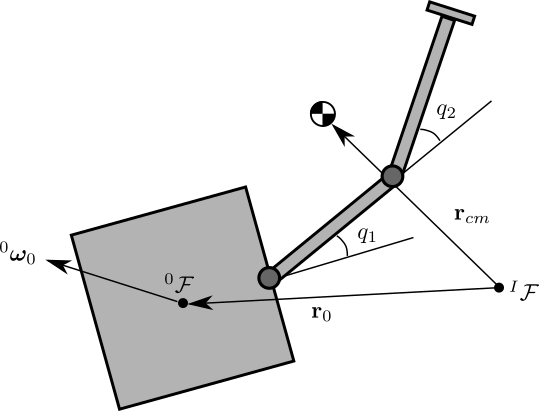
\includegraphics[width=0.5\textwidth]{system.png}
	\caption{The system sketch of a 2-link free-flying manipulator. The base is free to translate and rotate in the plane, resulting in a coupling between base and manipulator motion that is apparent in the manipulator equations.}
	\label{fig:sys}
\end{figure}

The base and the links have masses $\{m_0, .., m_n\}$ and moments of inertia $\{I_{zz,0}, .., I_{zz,n}\}$, in addition to center of mass positions $\{\mathbf{r}_{CM,0}, .., \mathbf{r}_{CM,n}\}$. Geometrically, the links have lengths from joint-to-joint of lengths $\{l_1, .., l_n\}$, with an initial manipulator offset $\mathbf{l}_0$ from the base CM.

The dynamics, presented here in manipulator equation form in equation \ref{eqn:dyn1} are given by Dubowsky using a Lagrangian derivation \cite{Dubowsky1993}. However, Dubowsky uses the system center of mass (CM) position rather than the base position in his formulation---this makes the form of $\mathbf{H}$ sparser, but is a bit less intuitive when describing the robot state.

\begin{equation}
\label{eqn:dyn1}
	\mathbf{H}(\mathbf{q})\dot{\mathbf{v}} + \mathbf{C}(\mathbf{q}, \omega_0, \dot{\mathbf{q}})\mathbf{v} = \bm{\tau}
\end{equation}

Above, $\mathbf{H}$ is the inertia matrix, $\mathbf{C}$ is the matrix containing nonlinear terms (e.g., Coriolis), and $\bm{\tau}$ is the control vector. Here, the control vector consists of the following:

\begin{align}
	\bm{\tau} = \begin{bmatrix} ^0\mathbf{F}_0^\top & ^0\bm{\tau}_0^\top & \bm{\tau}_q^\top \end{bmatrix}^\top \\
	\bm{\tau} = \begin{bmatrix} ^0F_1 & ^0F_2 & ^0\tau_0 & \tau_1 & \tau_2 \end{bmatrix}^\top
\end{align}

Note that the thruster forces could also easily be written in $^0\mathcal{F}$ via a frame transformation. For this scenario, $\mathbf{H}$ has the following form:

\begin{align}
\mathbf{H}(\mathbf{q})  = \begin{bmatrix} M \mathbf{I}_{2 \times 2} & \mathbf{M}_{r \omega} & \mathbf{M}_{r m} \\
\mathbf{M}_{r \omega}^\top & \mathbf{M}_{\omega} & \mathbf{M}_{\omega m} \\
\mathbf{M}_{r m}^\top &  \mathbf{M}_{\omega m}^\top & \mathbf{M}^{}_{m}\\
\end{bmatrix}\\
\end{align}


$M$ is the total system mass. $\mathbf{M}_{\omega} \in \mathbb{R}^{1 \times 1}$ contains terms affecting $\bm{\omega}$, $\mathbf{M}_{\omega m} \in \mathbb{R}^{1 \times n}$ is a coupling term that shows the effect of arm motion on base disturbance and $\mathbf{M}^{}_{m} \in \mathbb{R}^{n \times n}$ captures the self-disturbance of the arm. The remaining terms are due to using the satellite base CM, rather than the system CM. Alternatively, the entire dynamics can be summarized in the robot manipulator format of equation \ref{eqn:dyn}, with terms grouped to explicitly represent impacts on the base, `$0$', and on the manipulator, `$m$'. An additional $\mathbf{B}$ matrix is listed for mixing thruster outputs into force and torque commands, though it is not needed for this scenario.

A grappling scenario is considered, where some target has been grappled by the free-flyer and must be transported following some reference trajectory, $\mathbf{r}_{des}$. This results in uncertainty in equation \ref{eqn:dyn}, namely in the parameters involving the end effector. For simplicity and as a proof-of-concept, this formulation will consider a grappled \textit{point mass}, meaning that there is a single unknown parameter: $m_3$, the mass of the grappled point mass payload perched exactly on the end of link 2. Figure \ref{fig:sys2} shows this scenario, where the payload in (b) can be thought of as a point mass.

\begin{figure*}[htb!]
\begin{gather}
\label{eqn:dyn}
\begin{bmatrix} \textbf{M}_0 & \textbf{M}_{0m} \\
\textbf{M}_{0m}^\top & \textbf{M}_{m}\end{bmatrix}
\begin{bmatrix} \ddot{\mathbf{q}}_0 \\ \ddot{\mathbf{q}}_m\end{bmatrix}
+ \begin{bmatrix} \textbf{C}_0 & \textbf{C}_{0m} \\
\textbf{C}_{0m}^\top & \textbf{C}_{m}\end{bmatrix}
\begin{bmatrix} \dot{\mathbf{q}}_0 \\ \dot{\mathbf{q}}_m\end{bmatrix} = \begin{bmatrix} \bm{\tau}_0 \\ \bm{\tau}_m \end{bmatrix} +
\begin{bmatrix} \mathbf{B}_0 & \mathbf{B}_{0m} \\
\mathbf{B}_{0m}^\top & \mathbf{B}_{m} \\
\end{bmatrix} \begin{bmatrix} \mathbf{u}_0 \\ \mathbf{u}_m \end{bmatrix}
\end{gather}
\end{figure*}

\begin{figure}[htb!]
	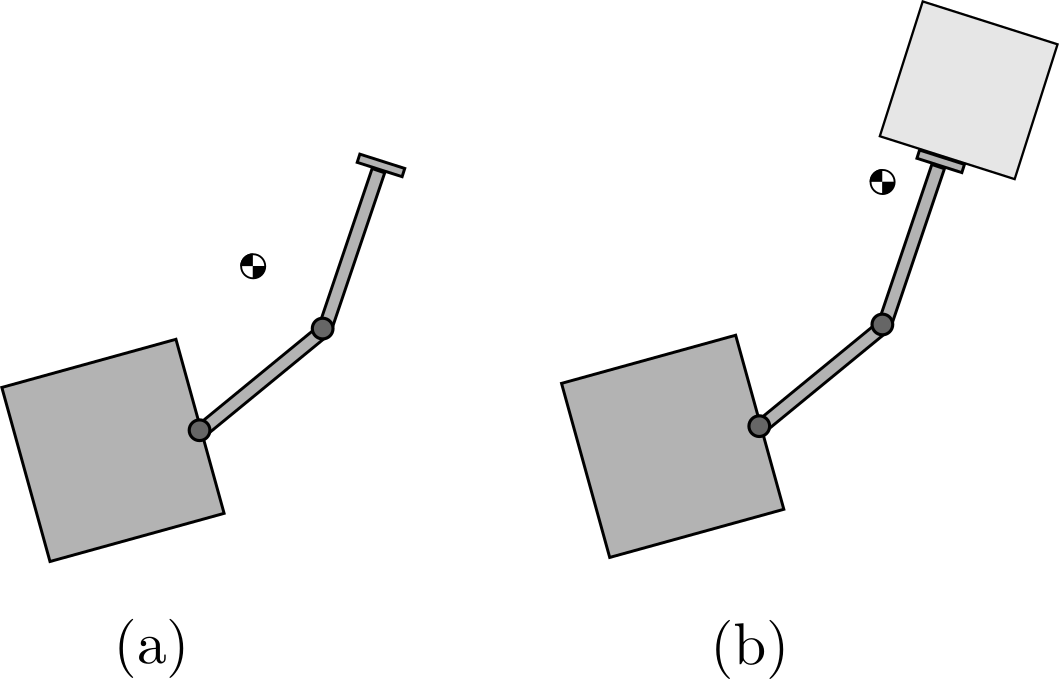
\includegraphics[width=0.5\textwidth]{grappled.png}
	\caption{In (a), the nominal system has a finely-tuned model and controller, accounting for the deterministic known parameters and free-flying dynamics. In (b), the system has grappled a payload of unknown mass, adding an unknown parameter to the model, $m_3$. The nominal system model has surely changed.}
		\label{fig:sys2}
\end{figure}


\section{APPROACH}
 
In order of increasing complexity, some control approaches for this problem include simple PD position control, trajectory control, and adaptive control. This build-up is also discussed in Chapter 9 of Slotine and Li \cite{Slotine}. Ultimately, the adaptive control formulation is desirable as it is the only formulation that can account for the modified system dynamics.
 
\subsection{Simple Position Control}

PD position control aims to achieve a specified state vector using feedback on the system positions and velocities. Essentially, the system can be thought to have ``virtual springs and dampers" that adjust its dynamics tune-ably based on the gain values and state reference. Proofs using virtual mechanical energy demonstrate that these systems are stable but may not have optimal tracking performance. For this system, a position controller is of the form may be used:

\begin{align}
	\bm{\tau} = -\mathbf{K}_p \mathbf{r}_{err} -\mathbf{K}_d \mathbf{v}_{err} &
\end{align}

Stability is assured for positive definite $\mathbf{K}$ matrices. Note that this is a slight modification of from pure position control, in that a reference trajectory of $\mathbf{v}$ is included.

\subsection{Trajectory Control}

Building on position control, it is possible to achieve better tracking performance if a control law respecting a trajectory (containing one derivative beyond the state vector) is produced. For nonlinear systems, this is often accomplished via feedback linearization such that system accelerations follow ones prescribed. However, this assumes exact knowledge of the dynamics.

Using the manipulator dynamics of equation \ref{eqn:dyn} and rearranging, a trajectory control strategy can be produced via:

\begin{align}
	\bm{\tau} = \mathbf{C}\mathbf{v} + \mathbf{H}\lbrack -\mathbf{K}_p \mathbf{r}_{err} -\mathbf{K}_d \mathbf{v}_{err} + \dot{\mathbf{v}}_{des} \rbrack&
\end{align}

Note that a reference acceleration must be designated via this procedure, $\dot{\mathbf{v}_{des}}$. The gain matrices may be tweaked as before for differing system performance.

\subsection{Adaptive Control}

But what if there is uncertainty or a change in the system assumptions? One approach is to compute reference trajectories fast enough such that these reference trajectories are themselves a method of control, called model predictive control (MPC). However, real-time computation is sometimes infeasible and nonlinear variants offer scant guarantees on robustness or convergence \cite{Rybus2017}. Tube-based robust MPC is being explored further for this purpose \cite{Lopez2019} \cite{Mammarella2018}. However, traditional reference-tracking control with guarantees on performance may be desirable.

Adaptive control, which uses sliding mode control to adapt parameters online and converge to a sliding surface is appropriate. Previous investigations using adaptive control for space applications have been demonstrated for both rigid and flexible link manipulators, though notably with only \textit{fixed bases} in \cite{Ulrich2010} \cite{Ulrich2012}. However, work by Senda et al. first adapted some of the developments by Slotine and Li to free-flying adaptive control. In the late 1990s, Guelman et al. simplified the task of parameter estimation to require only estimation of the \textit{relative influence} of grappled payload on the dynamics. Notably, other interesting approaches consider e.g., multiple arms or other control methods \cite{Jia2014}.

However, these approaches rarely provide a full view of their dynamics and controller formulations which is unfortunate particularly for Senda et al. Senda's approach uses an adaptive control approach based directly on Slotine's fixed-base adaptive controller, which relies on a linear parameterization of the dynamics in terms of the adaptation parameters \cite{Slotine}. However, the free-flying dynamics are much more complicated and higher-dimensional than the fixed-base dynamics, so determining reasonable parameterizations is extremely challenging (if even feasible). Senda does not discuss these details and presents some limited 2D simulations.

An adaptive controller similar to Senda's and the generic manipulator equation formulation of Slotine and Li is presented here, with an attempt at linear parameterization. The uncertain parameter vector, $\mathbf{a}$ is simply 
 
\begin{align}
	a &= \lbrack m_3 \rbrack
\end{align}
 
 An adaptation and control law must be produced so that the unknown parameters can be tweaked during operation. Assuming linearly parameterized dynamics, a sliding control approach can be taken. For a 2nd order system, a sliding variable $\mathbf{s}$ is introduced:
 
 \begin{align}
 	\mathbf{s} = \mathbf{v}_{err} + 2 \lambda_0 \mathbf{r}_{err}
 \end{align}
 
 where $\lambda$ is used to define convergence on the sliding surface. Reference values of $\dot{\mathbf{v}}_r$ and ${\mathbf{v}}_r$ are produced according to the desired trajectory and current tracking error:
 
 \begin{align}
 	\dot{\mathbf{v}}_r &= \dot{\mathbf{v}}_{des} - 2\lambda_0 \dot{\mathbf{e}}\\
 	\mathbf{v}_r &= \mathbf{v}_{des} - 2\lambda_0 \dot{\mathbf{e}}
 \end{align}
 
 The next step is choosing a set of parameters (perhaps more complex than the actual underlying uncertain parameter(s)) that can be linearly combined with nonlinear functions to produce $\dot{\mathbf{v}}$. For this 10-dimensional nonlinear system, this is a real challenge. The approach taken here uses the MATLAB Symbolic Toolbox to group nonlinear terms and separate out just $m_3$---however, this still leaves $m_3$ within the nonlinear terms. This work simply leaves $m_3$ within the parameter vector and uses the latest estimate $\hat{a}$, and using the resulting matrix for adaptation. This likely forfeits convergence guarantees of the approach, though a more in-depth analysis is required. It would also be worth looking into other choices of adaptation parameters that might allow for a linear parameterization of the plant dynamics. The quasi-parameterization can be written:
 
 \begin{align}
 	\mathbf{H}(\mathbf{q})\dot{\mathbf{v}_r} + \mathbf{C}(\mathbf{q}, \omega_0, \dot{\mathbf{q}})\mathbf{v}_r = \mathbf{Y}(\mathbf{r},\mathbf{v},\mathbf{v}_r,\dot{\mathbf{v}}_r, \hat{a})a
 \end{align}

A control law to feedforward based on the best estimate, along with feedback on the converging sliding variable, is given as equation \ref{eqn:slide} with accompanying adaptation law equation \ref{eqn:adapt}:

 \begin{align}
	\bm{\tau} &= \mathbf{Y}\hat{a} - \mathbf{K}_D\mathbf{s}\\
	\label{eqn:slide}
	\dot{\hat{a}} &= -\Gamma\mathbf{Y}^\top\mathbf{s}\\
	\label{eqn:adapt}
\end{align}

where $\Gamma$ influences adaptation rate and $\mathbf{K}_D$ is used to show Lyapunov convergence. However, a more detailed convergence analysis is necessary since $\mathbf{Y}$ is a function of $\hat{a}$ here.

\section{RESULTS}

The free-flying manipulator dynamics were implemented in MATLAB, using a wrapped version of the Spacecraft Robotics Toolkit (SPART) for the forward dynamics. \cite{Virgili-Llop} MATLAB's ODE23 numerical integration tool was used for system propagation: the reference trajectory and adaptive tracking controller were integrated into this framework. The analysis here is for unconstrained motion, though one could conceivably create more complicated reference trajectories or use a real-time control approach that considers e.g., obstacle constraints.

Reference trajectories were created for a simple step-response, and a more complex base movement with sinusoidal arm movements. Only results from the complex movement are shown here. The full trajectory was obtained using simple finite differencing of the prescribed position commands. Both of these trajectories were tested with tuned versions of the aforementioned controllers. Finally, the complex trajectory was tested using the controllers with modified inertial properties due to grappling an object: these modified properties were not known beforehand, so gains (and parameter estimates) are unchanged, with the notable exception of the adaptive controller. The reference trajectories are made ``sufficiently fast" so that model error and nonlinearity becomes significant in system performance. 

For both cases, $m_0 = 10 $ kg, $m_1 = m_2 = 1$ kg, $I_{zz,0} = 0.1$ kg$^2$-m$^4$, $I_{zz,1} = I_{zz,2} = 0.05$ kg$^2$-m$^4$ with $l_1 = l_2 = 0.3$ m, with CM at the link centroids. However, for the modified case a new mass is added to the end of link 2, with $m_3 = 8$ kg, a significant mass fraction compared to the base.

\subsection{Simple Position Control}

The PD controller was tuned for the nominal case, but does not have perfect tracking---it is only a position/velocity controller and cannot account for nonlinearities.

\begin{figure*}[h!]
	\centering
	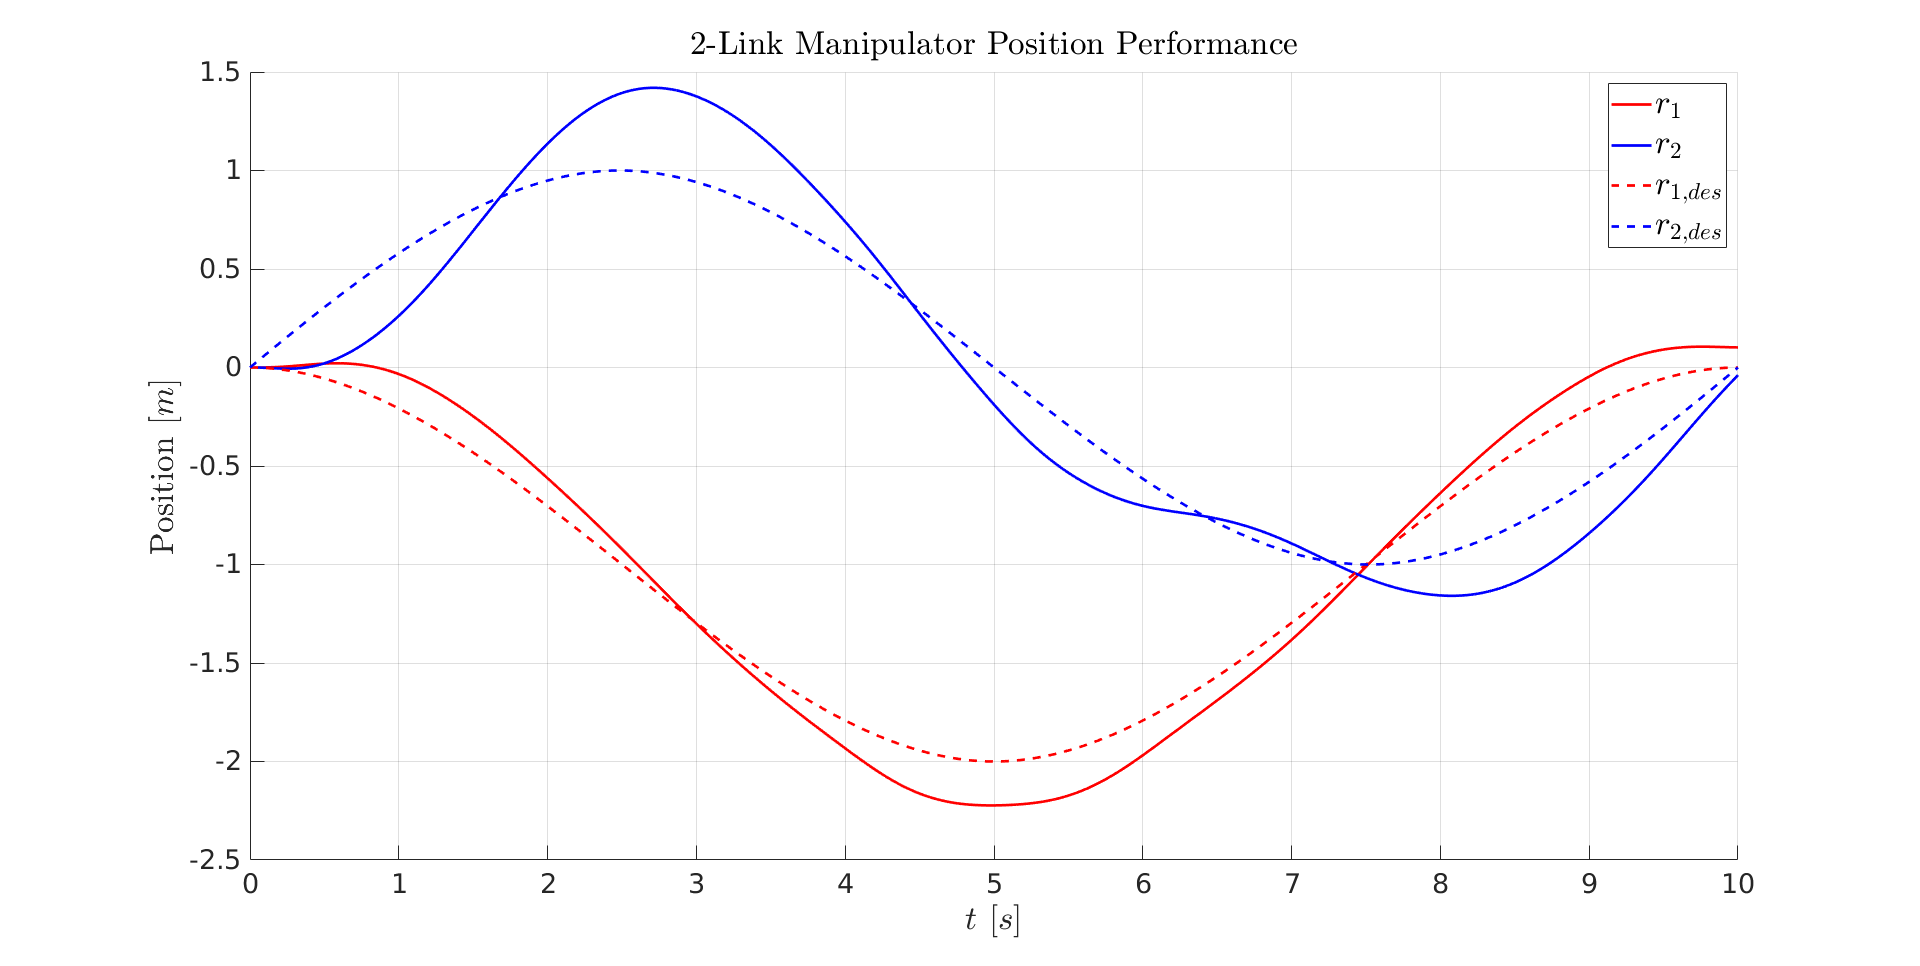
\includegraphics[width=0.9\textwidth]{pd_pos_1.png}
	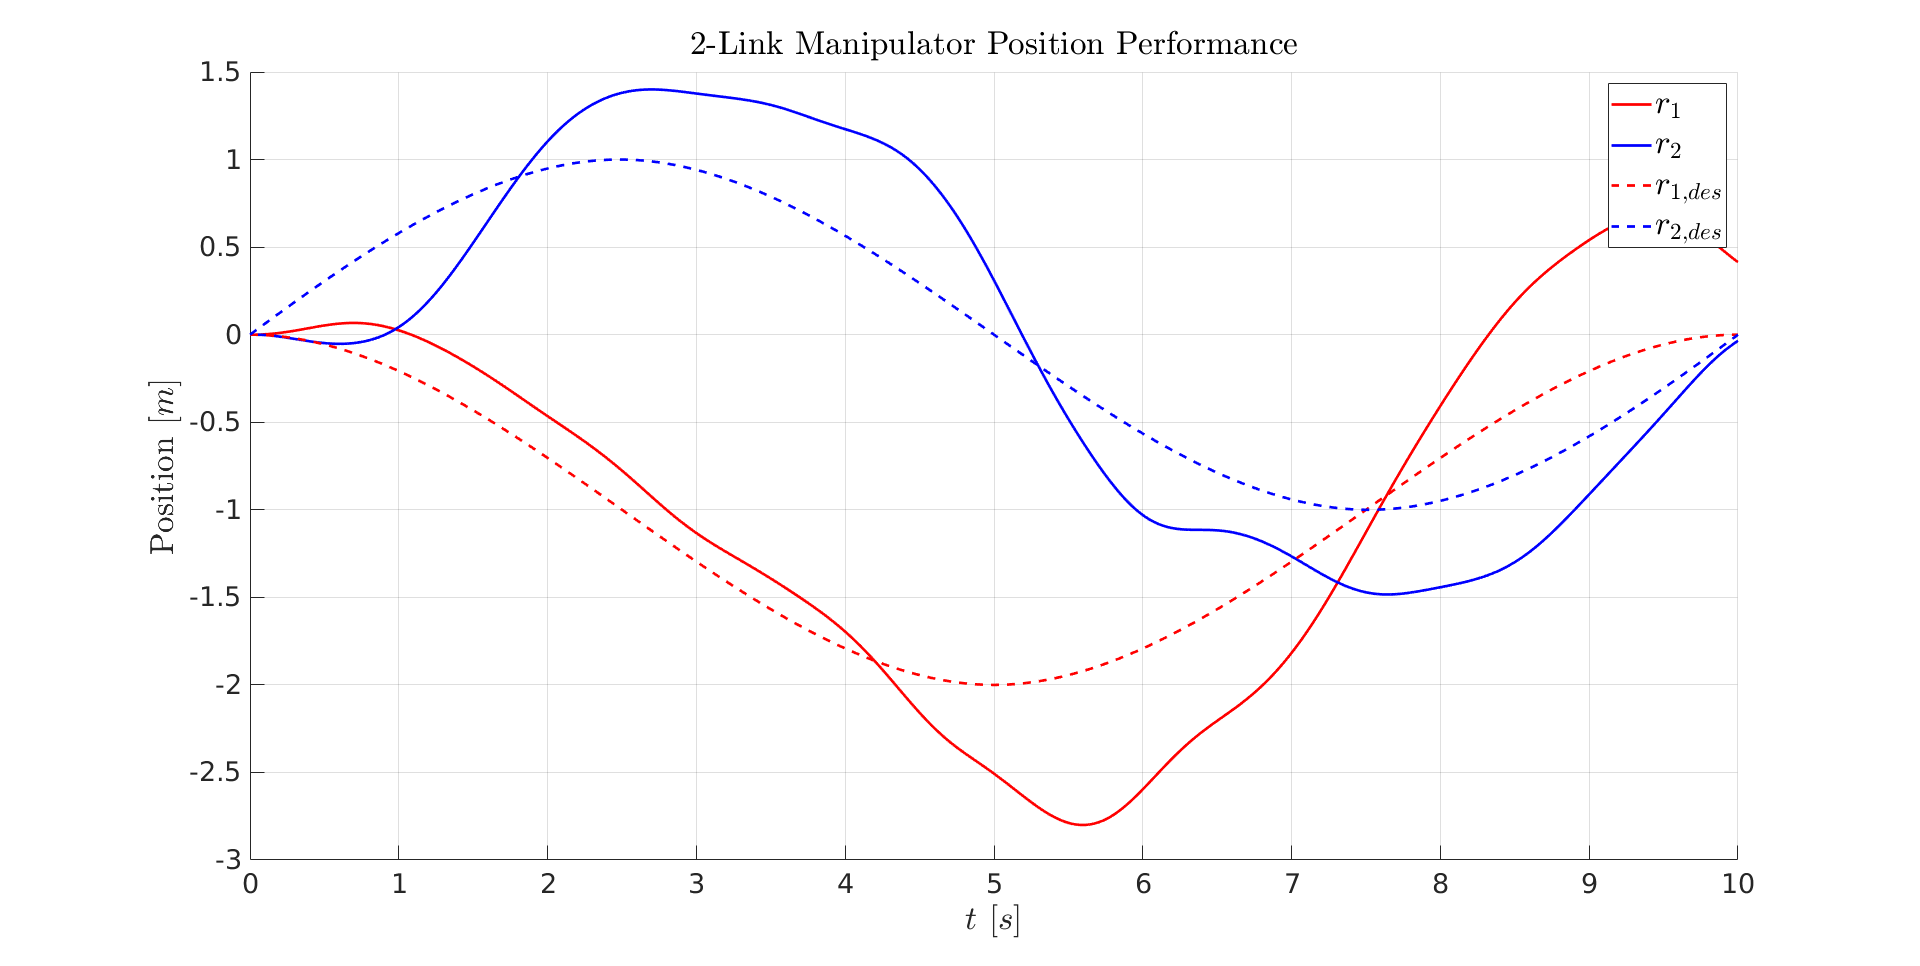
\includegraphics[width=0.9\textwidth]{pd_pos_2.png}\\
	\caption{This is a tiger.}
\end{figure*}

\begin{figure*}[h!]
	\centering
	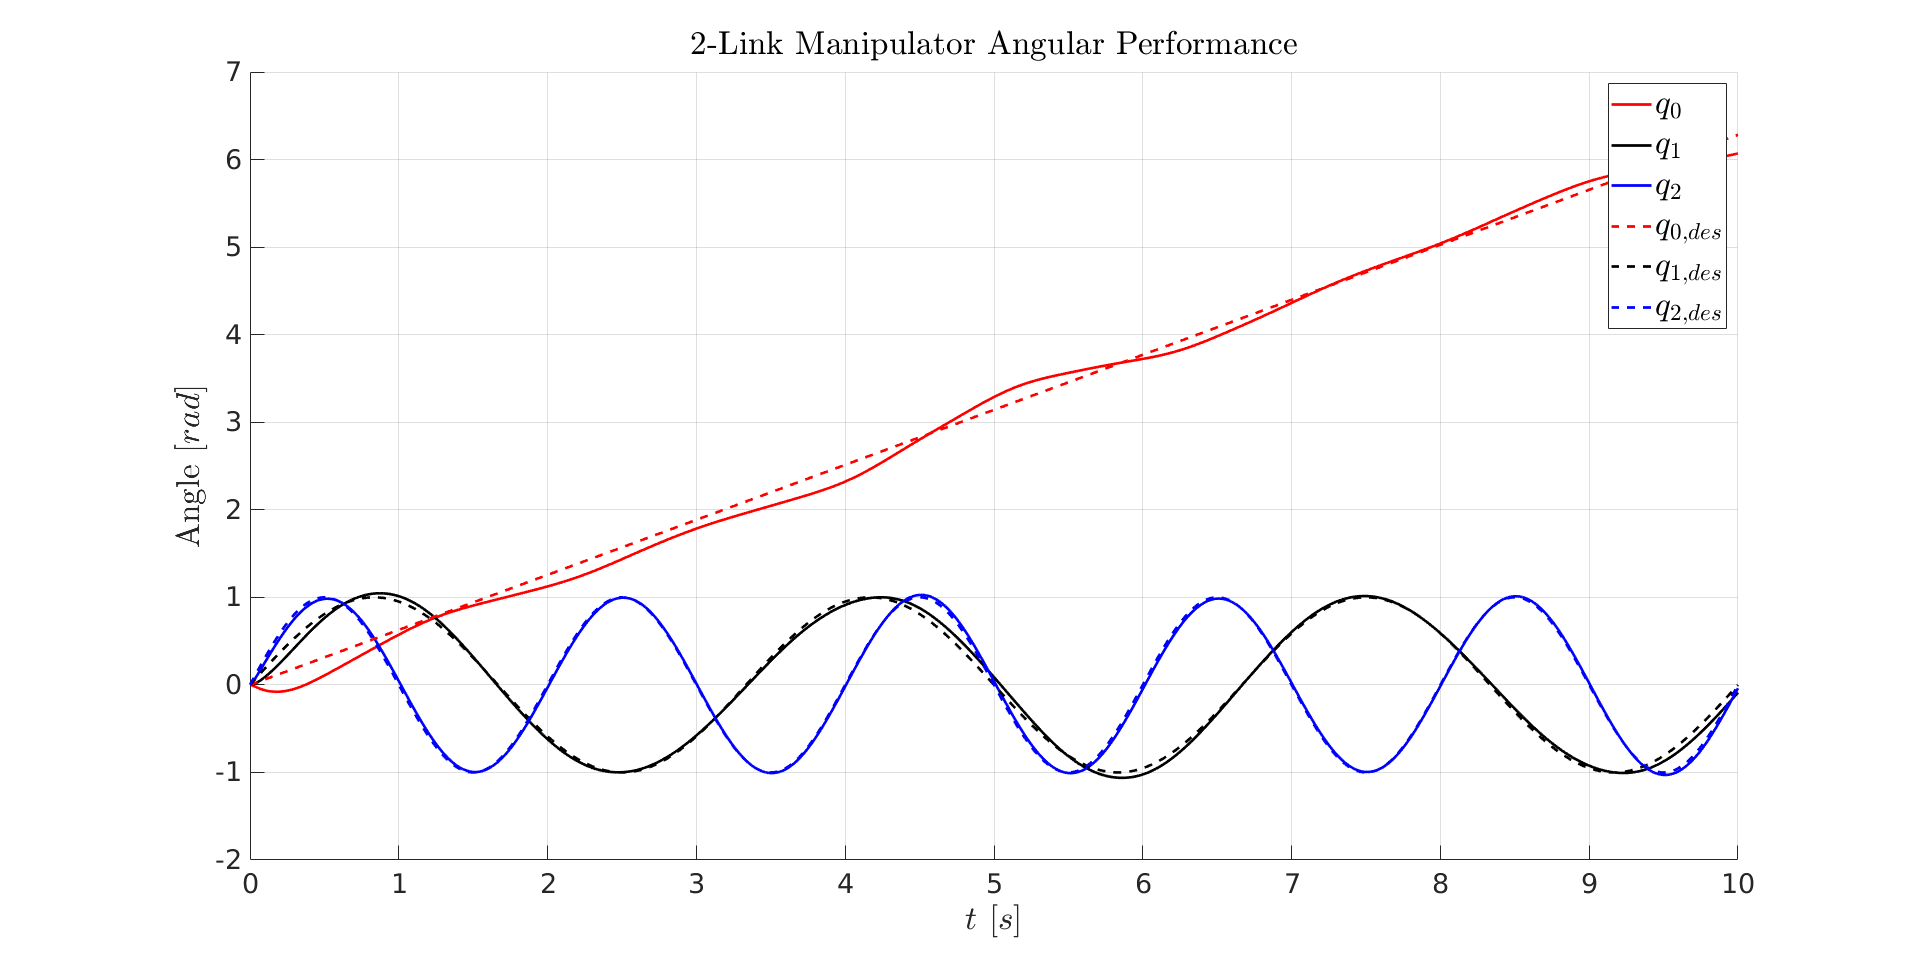
\includegraphics[width=0.9\textwidth]{pd_ang_1.png}
	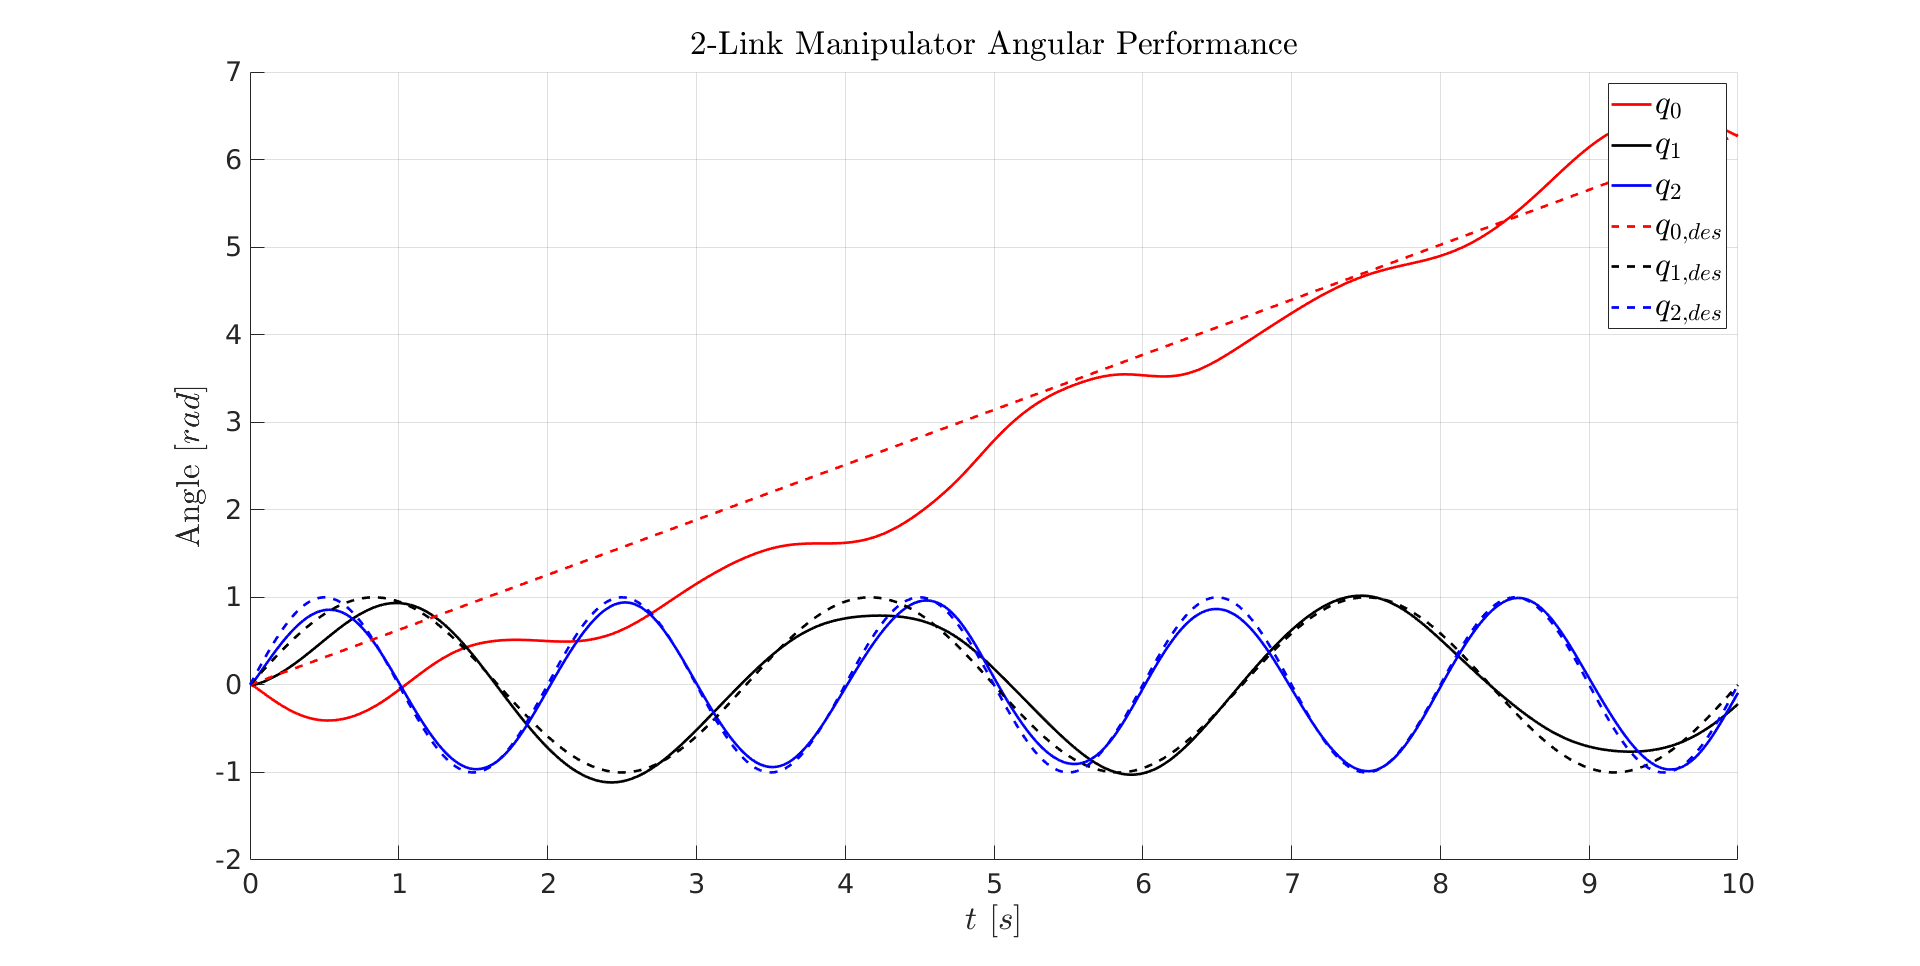
\includegraphics[width=0.9\textwidth]{pd_ang_2.png}
	\caption{This is a tiger.}
\end{figure*}

\begin{figure*}[h!]
	\centering
	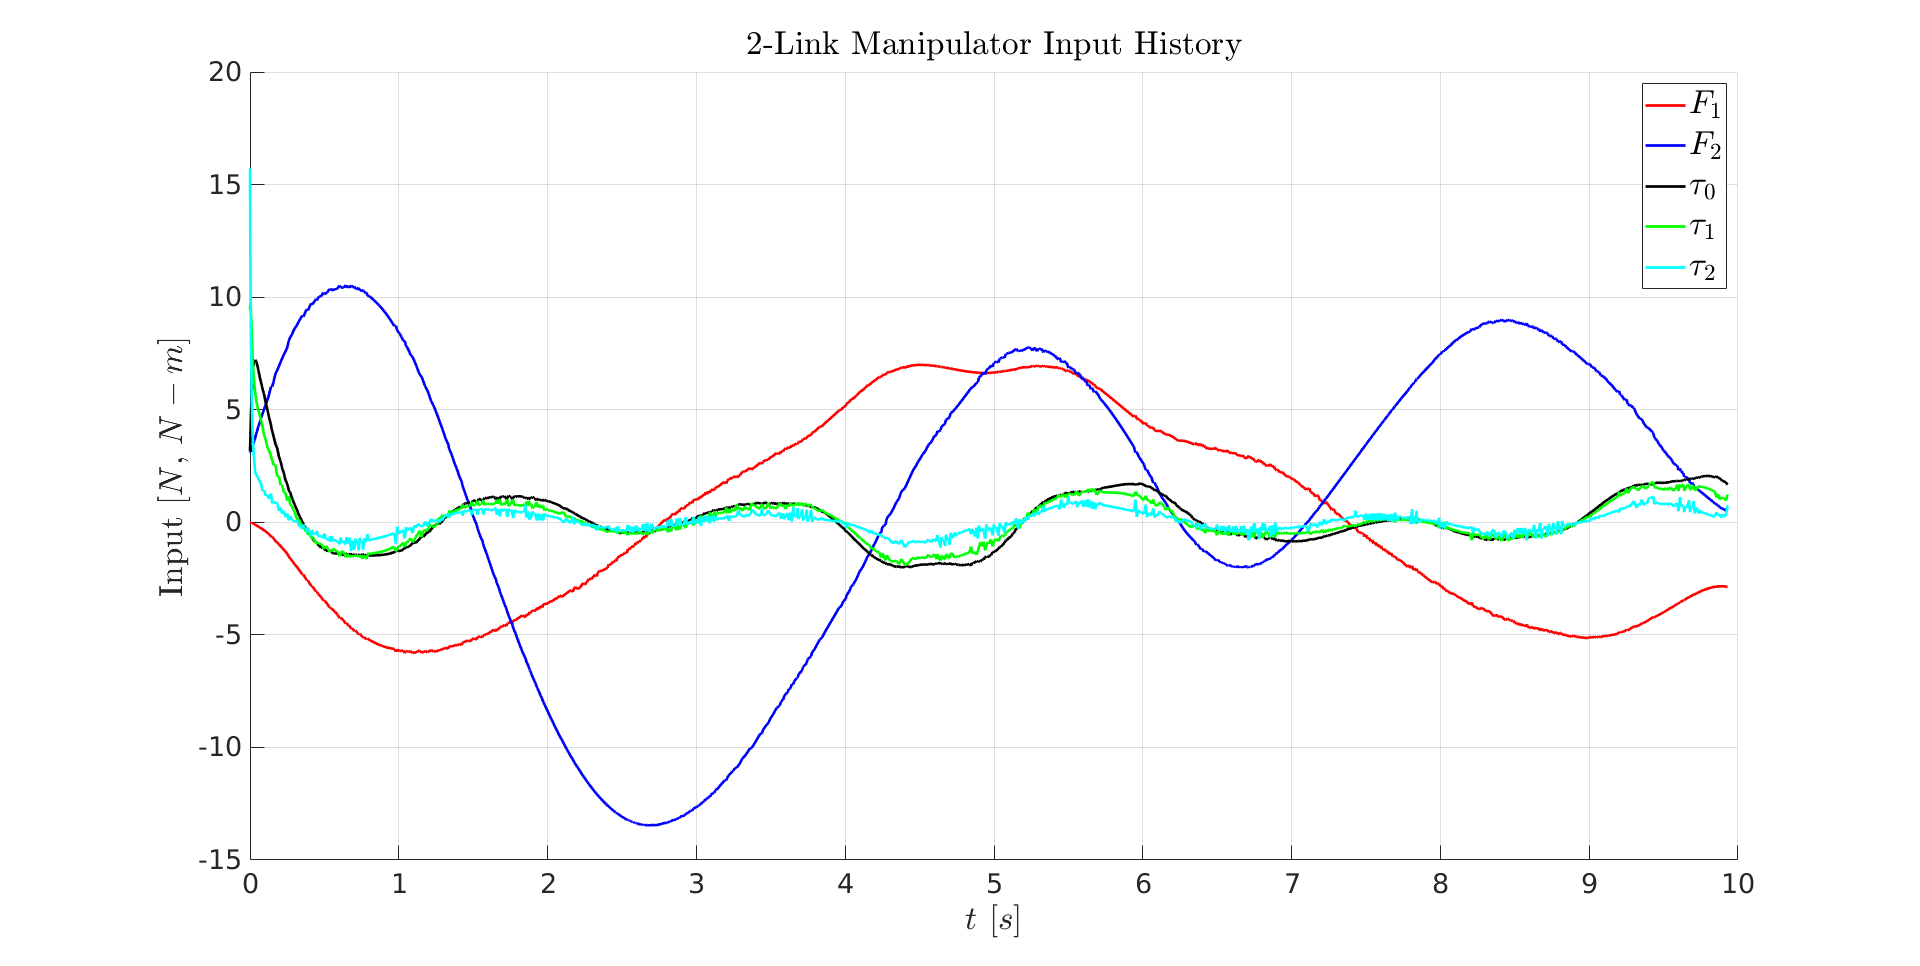
\includegraphics[width=0.9\textwidth]{pd_u_1.png}
	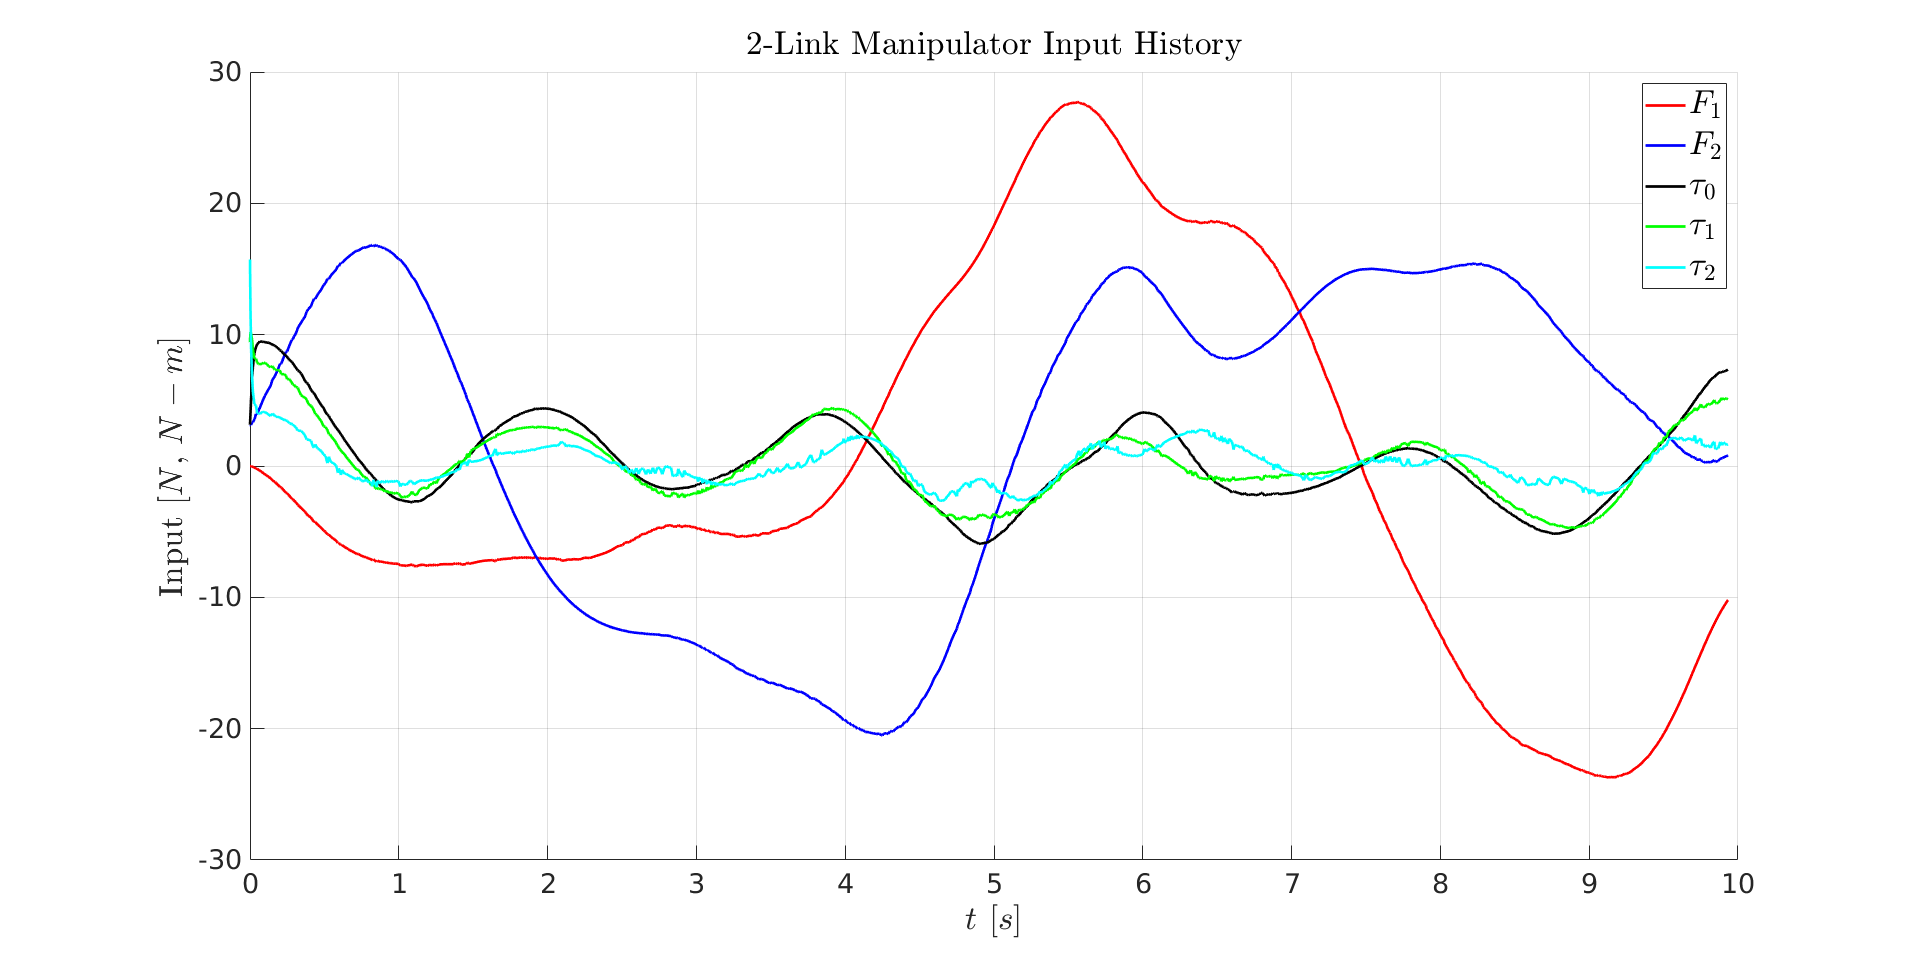
\includegraphics[width=0.9\textwidth]{pd_u_2.png}
	\caption{This is a tiger.}
\end{figure*}



\subsection{Trajectory Control}

The trajectory controller was also tuned for nominal tracking performance.

\begin{figure*}[]
	\centering
	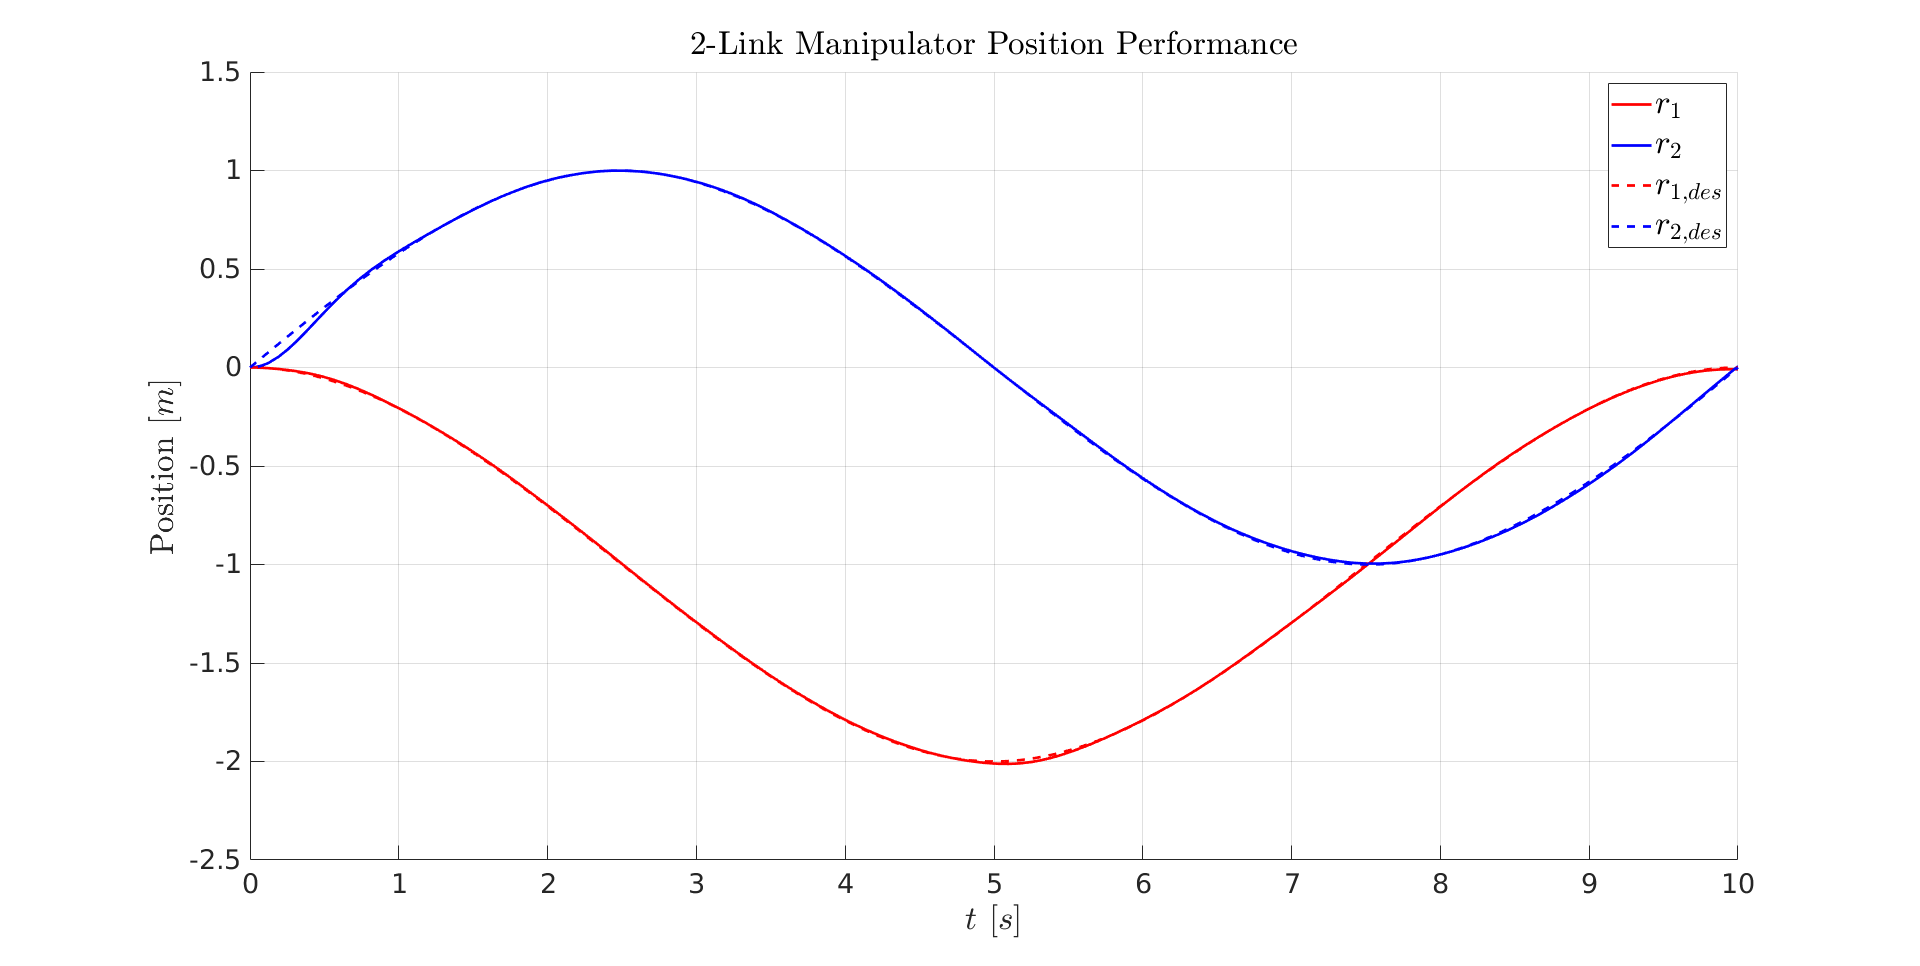
\includegraphics[width=0.9\textwidth]{fl_pos_1.png}
	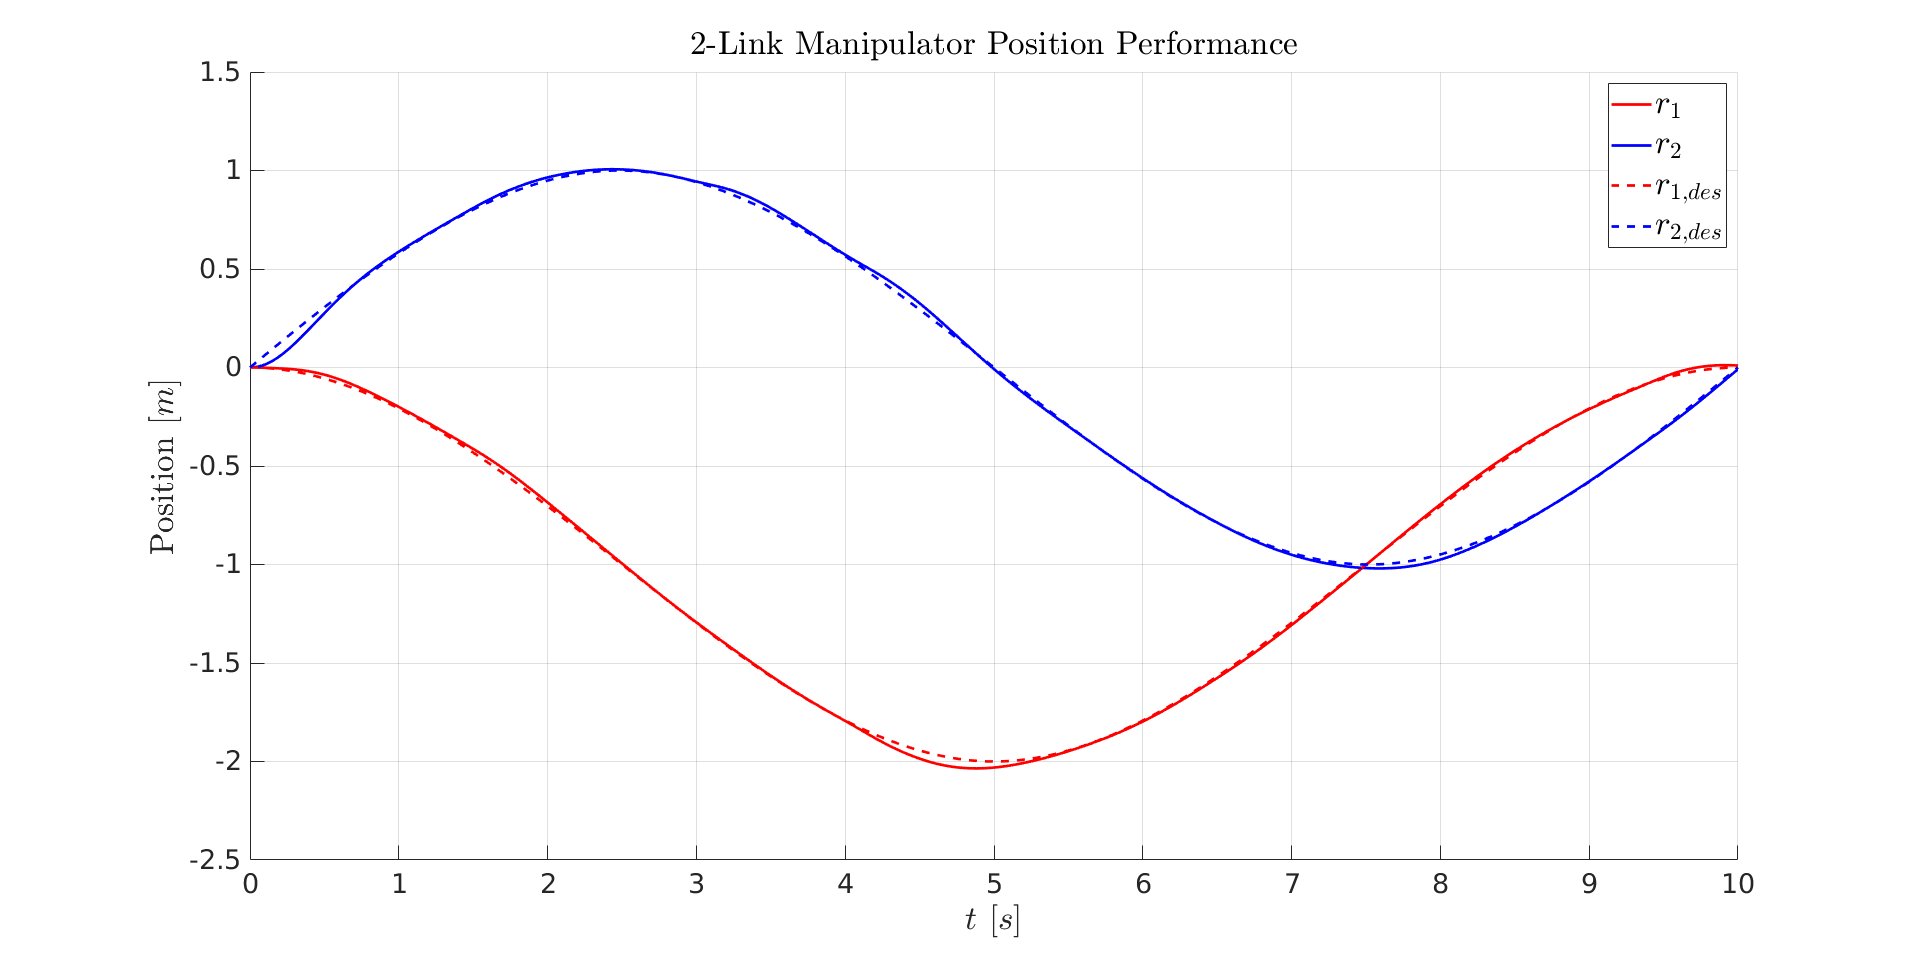
\includegraphics[width=0.9\textwidth]{fl_pos_2.png}\\
	\caption{This is a tiger.}
\end{figure*}

\begin{figure*}[]
	\centering
	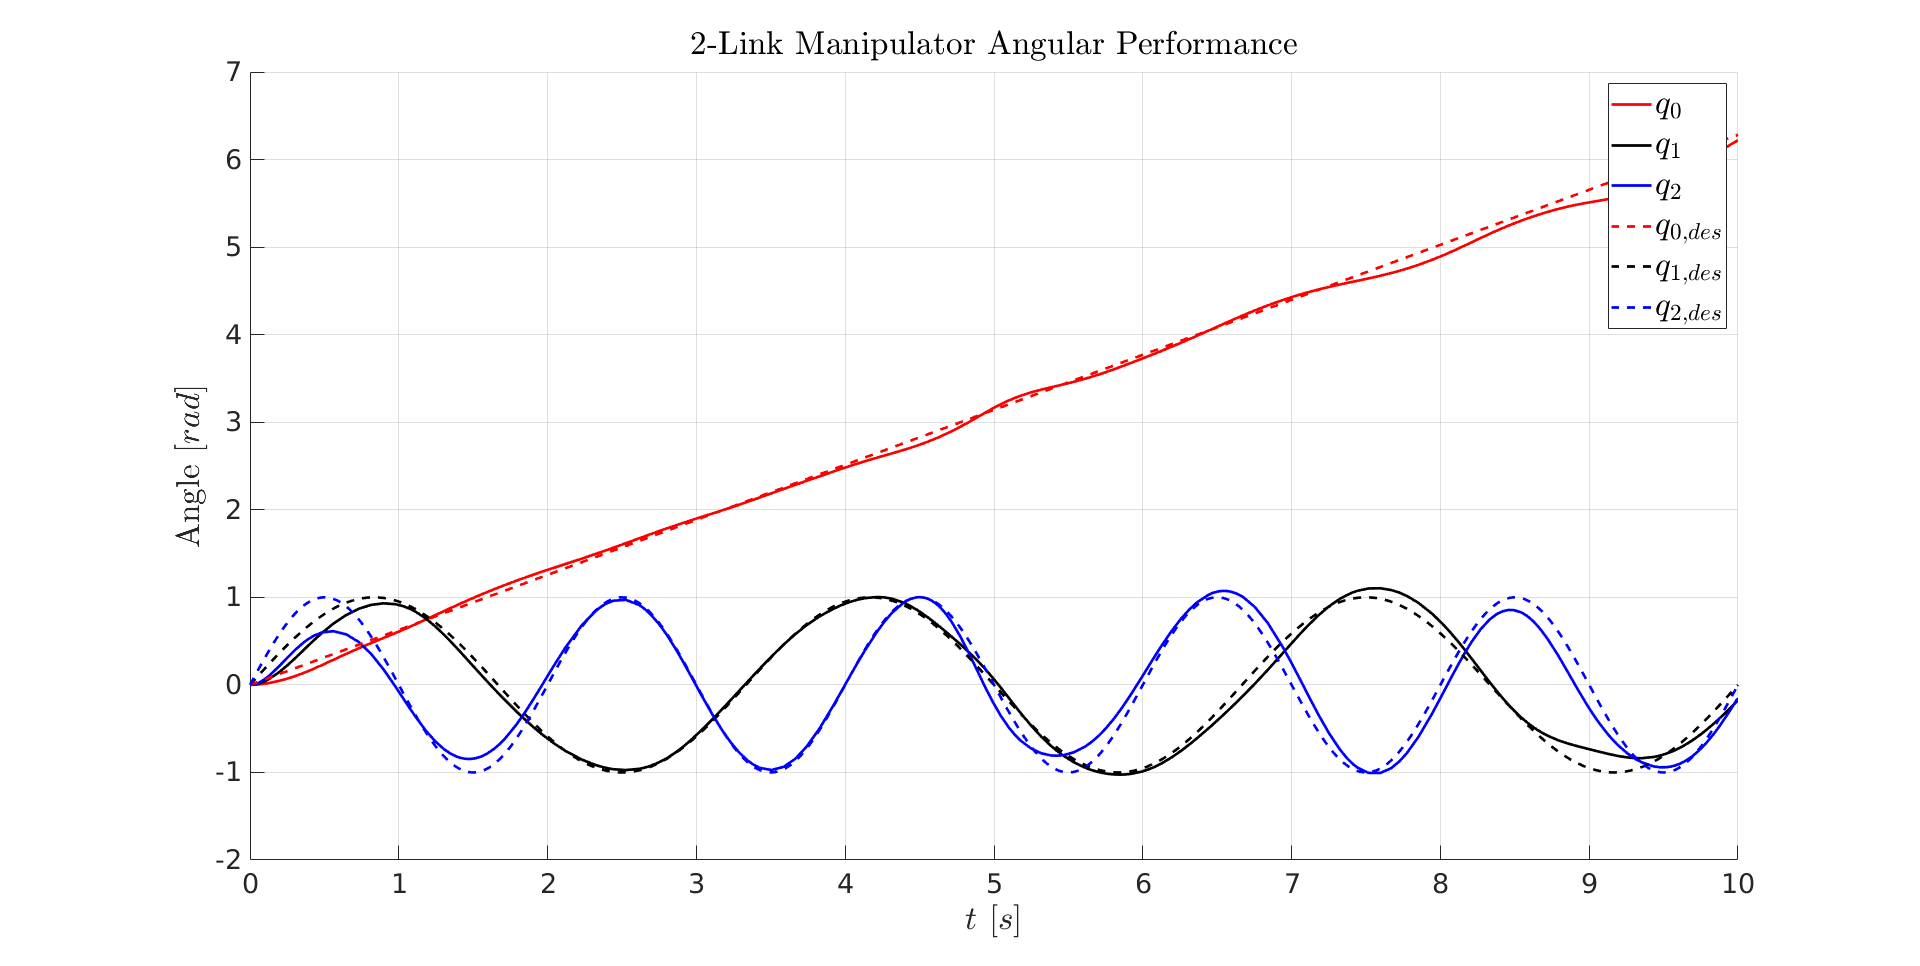
\includegraphics[width=0.9\textwidth]{fl_ang_1.png}
	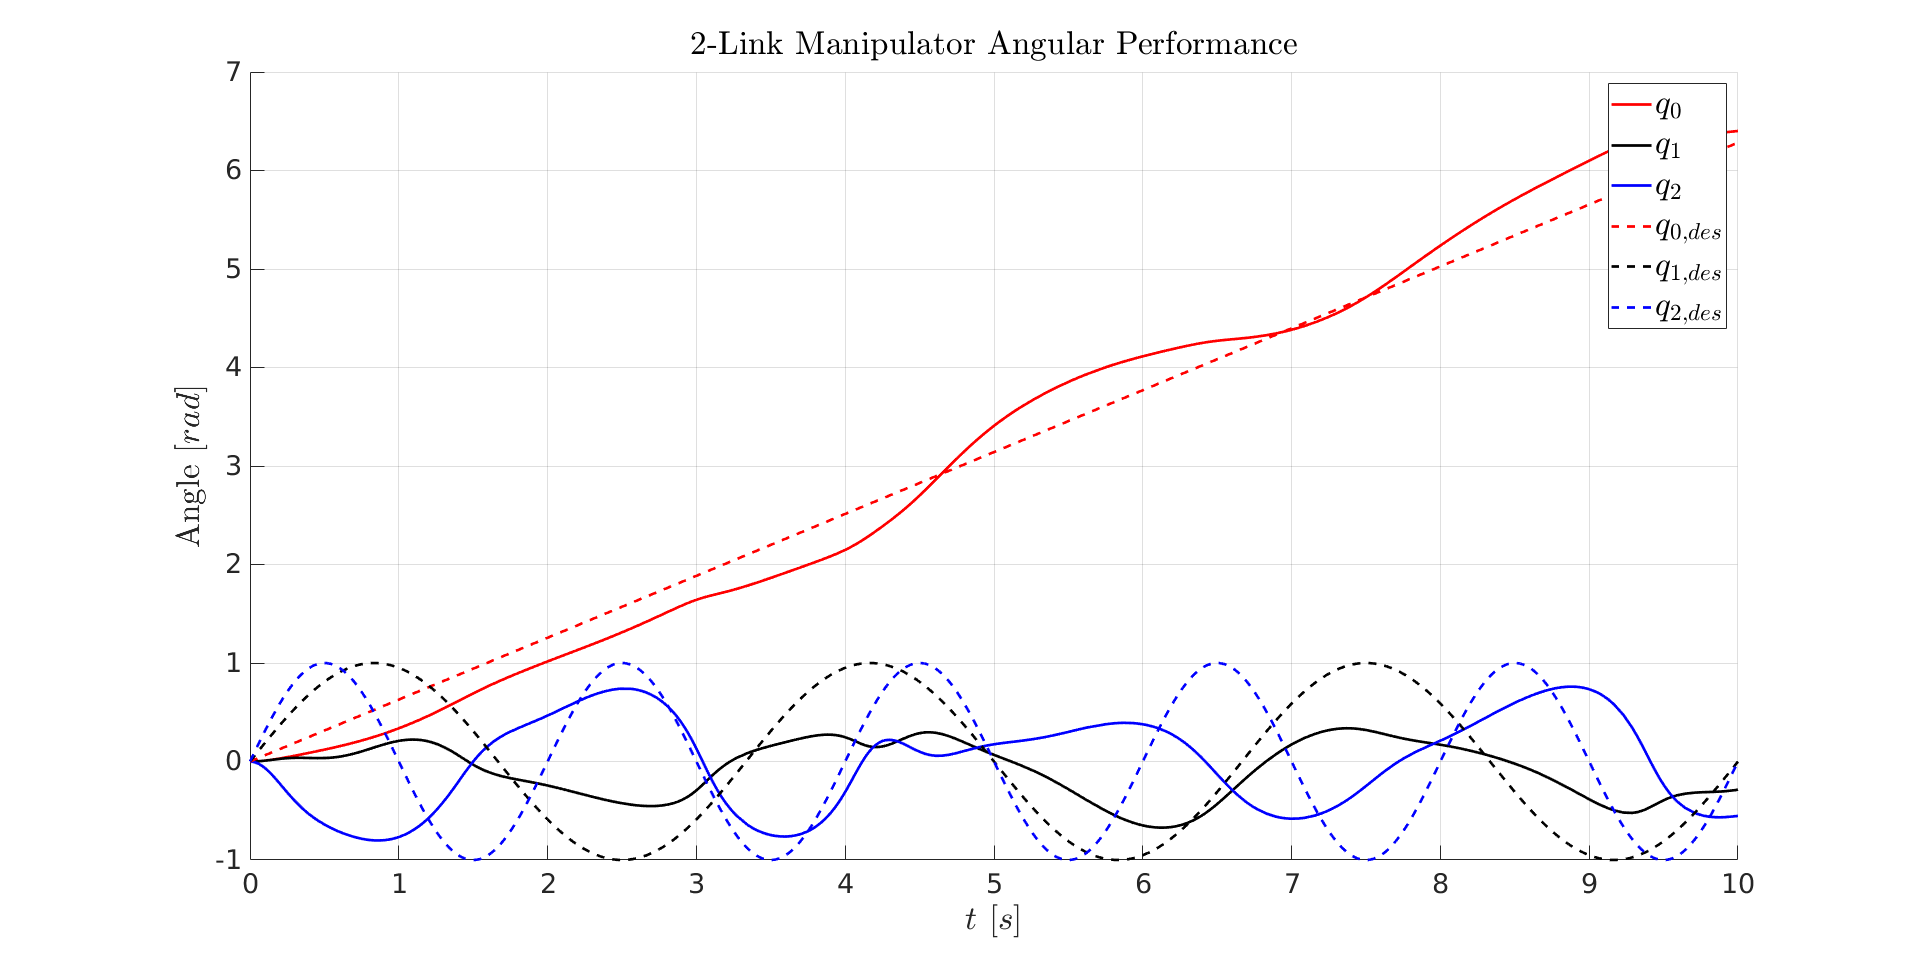
\includegraphics[width=0.9\textwidth]{fl_ang_2.png}
	\caption{This is a tiger.}
\end{figure*}

\begin{figure*}[]
	\centering
	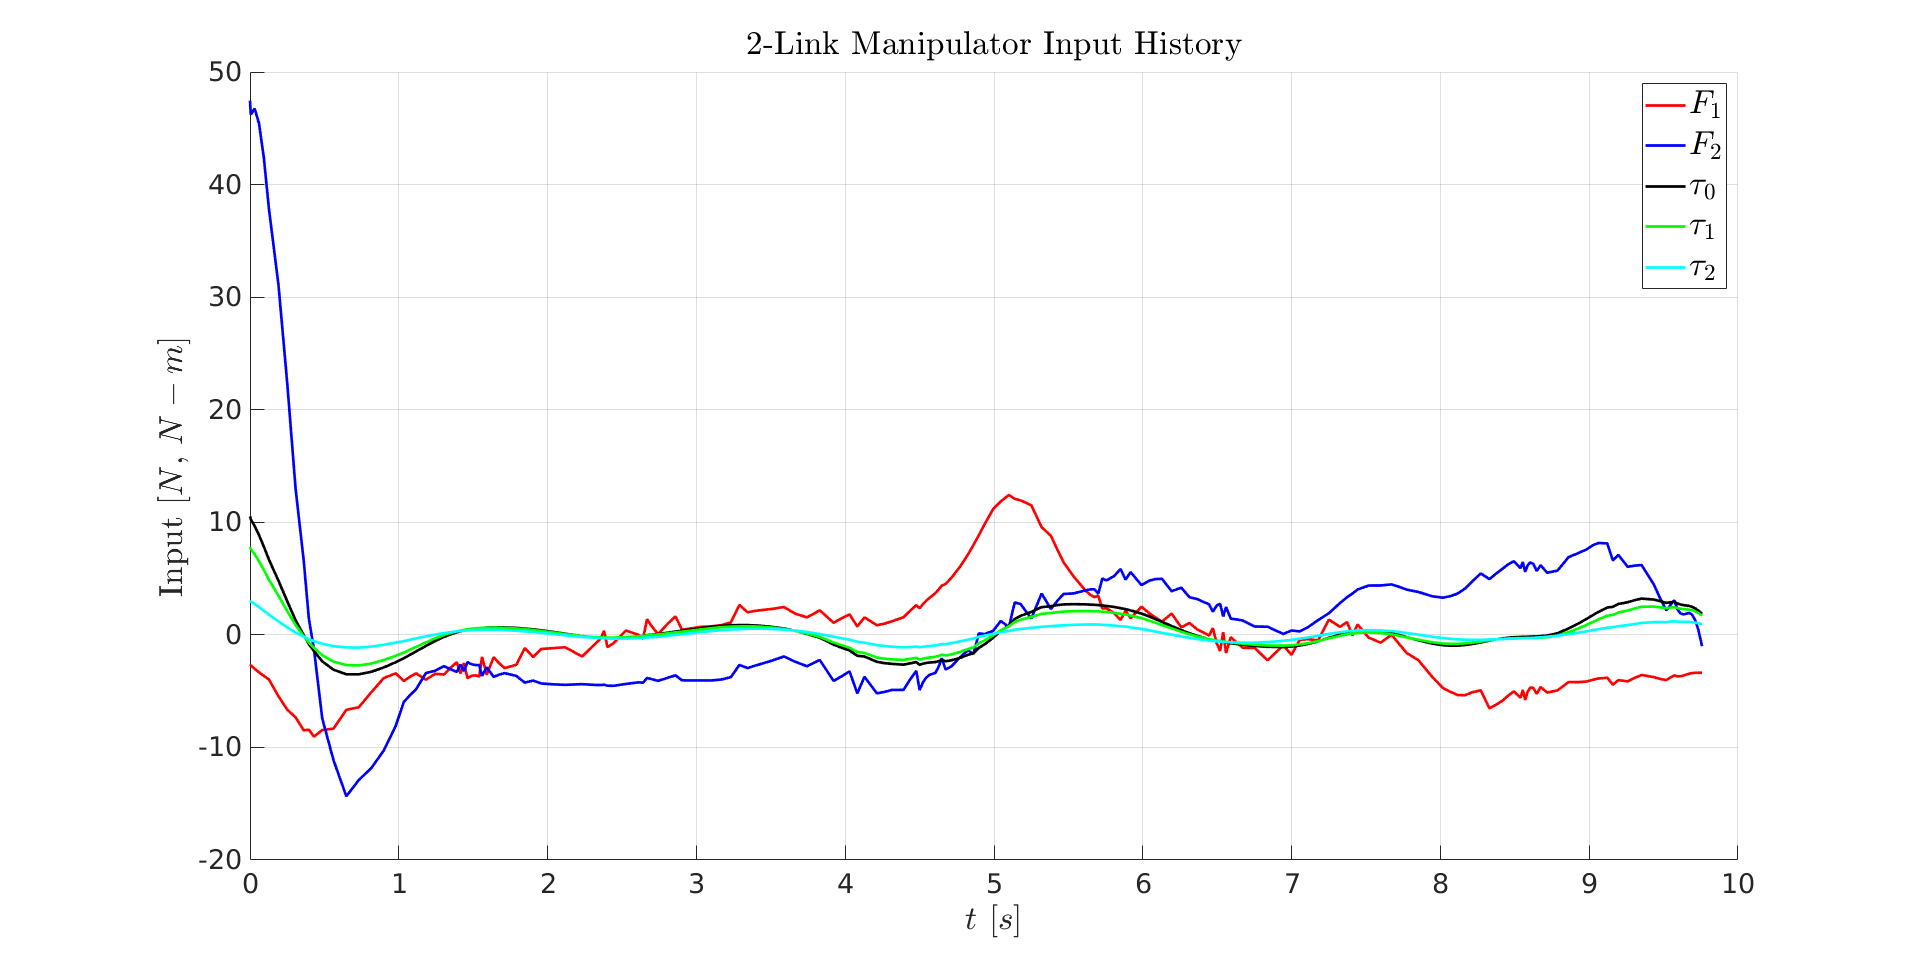
\includegraphics[width=0.9\textwidth]{fl_u_1.png}
	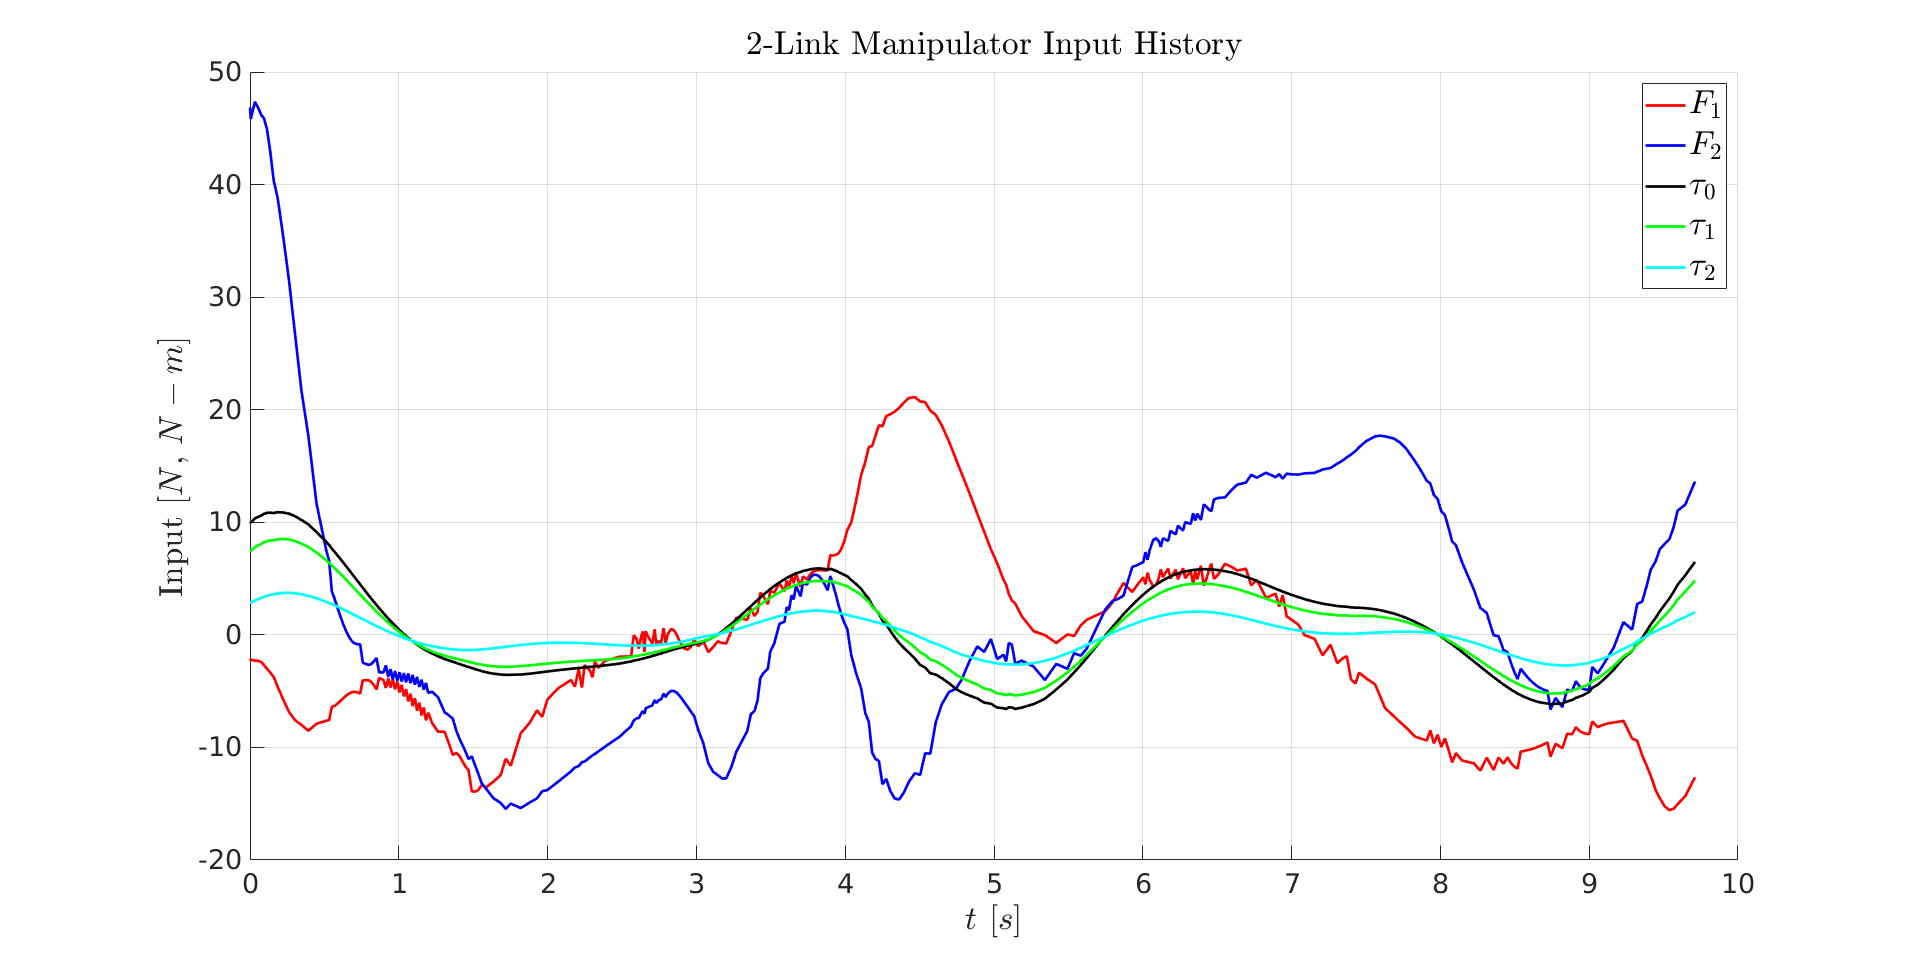
\includegraphics[width=0.9\textwidth]{fl_u_2.png}
	\caption{This is a tiger.}
\end{figure*}

\subsection{Adaptive Control}

The adaptive controller was the only controller used that had the ability to actively compensation for the change in mass parameters.

\begin{figure}[htb!]
	\centering
	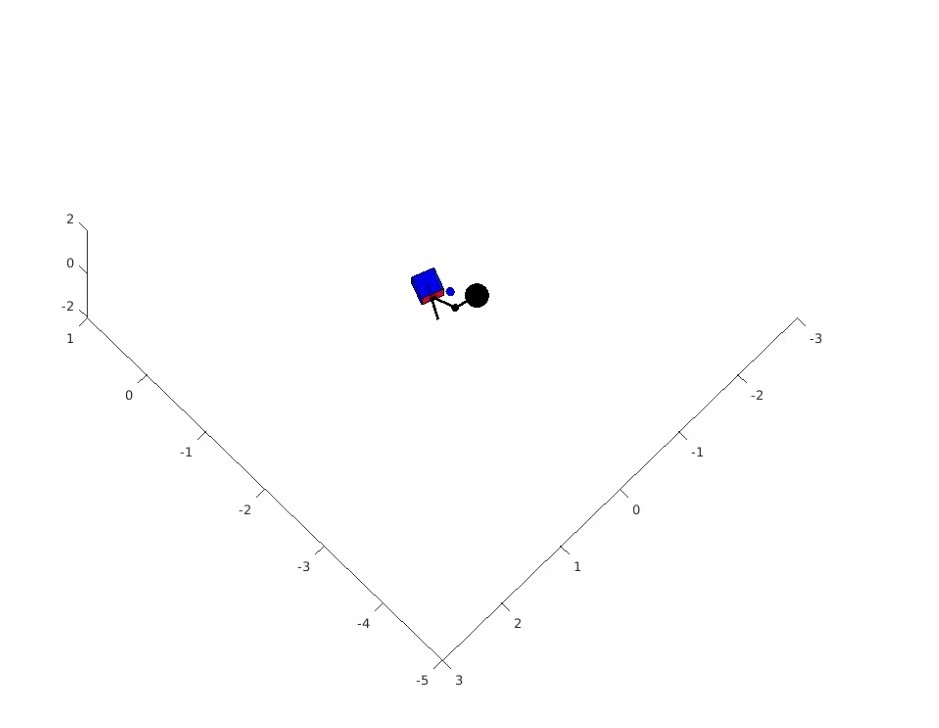
\includegraphics[width=0.5\textwidth]{visual.jpg}
	\caption{This is a tiger.}
\end{figure}

\begin{figure*}[]
	\centering
	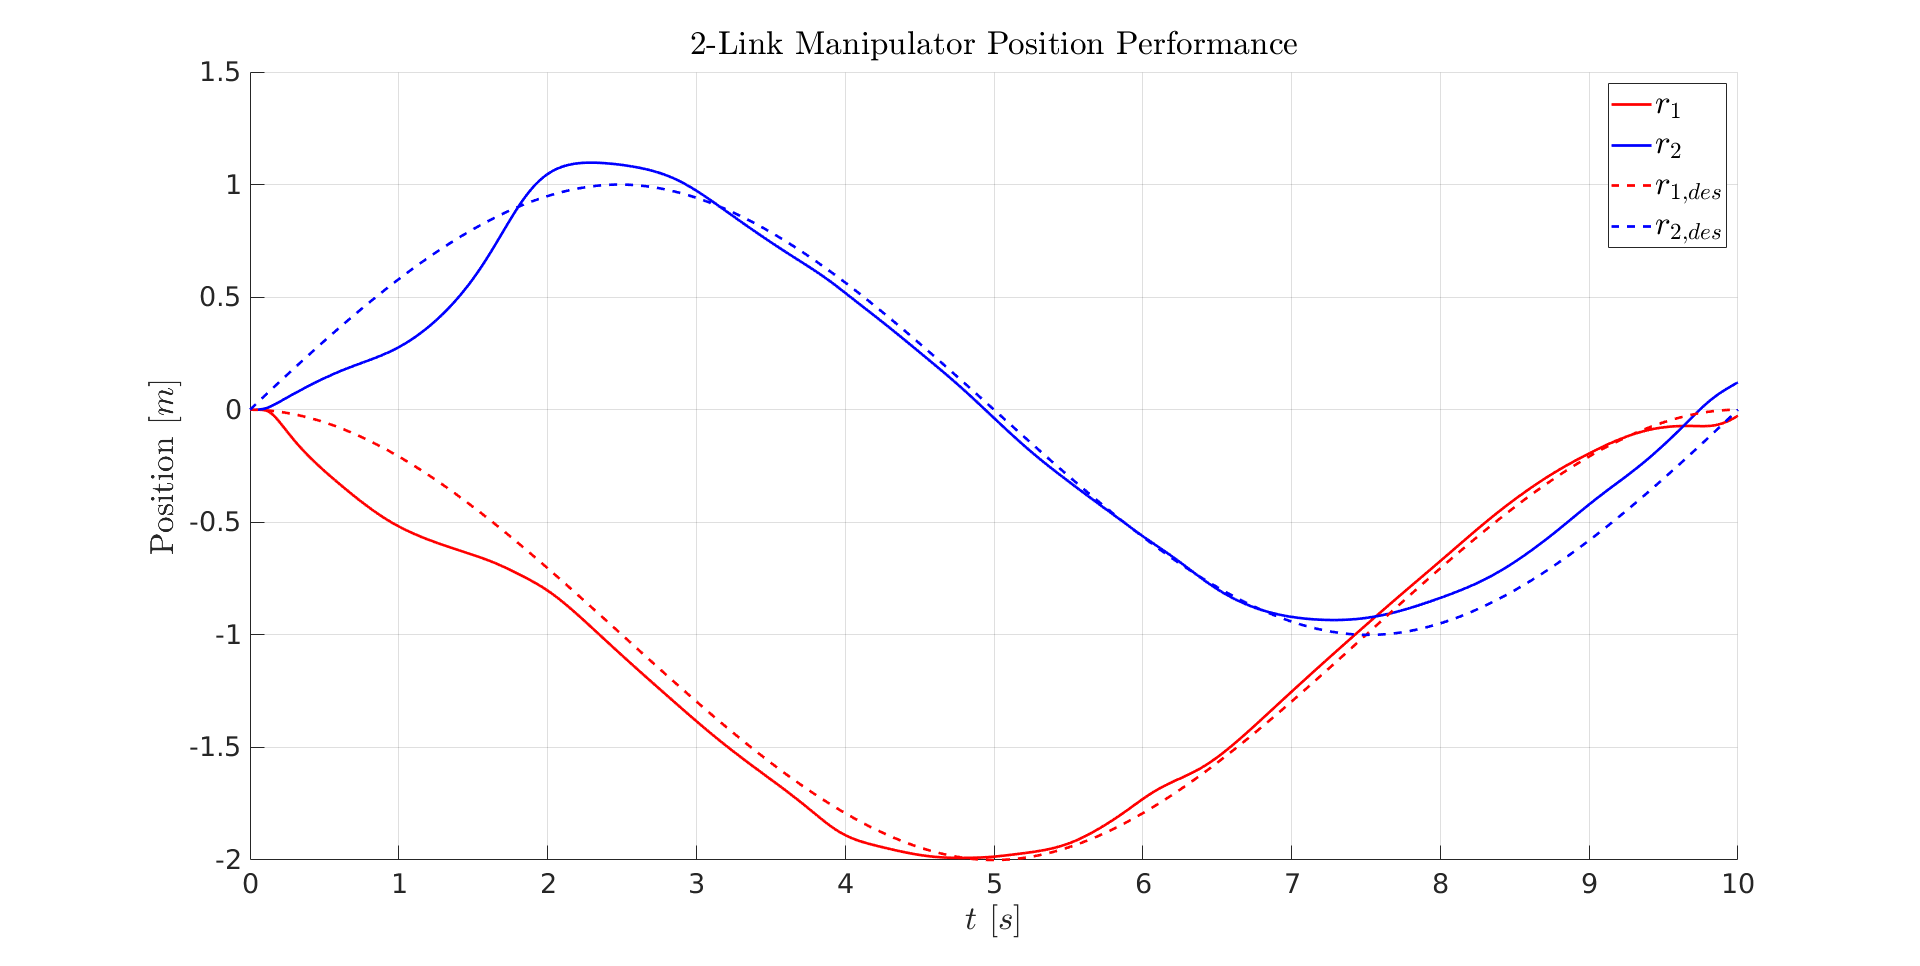
\includegraphics[width=0.9\textwidth]{ad_pos_2.png}
	\caption{This is a tiger.}
\end{figure*}
\begin{figure*}[]
	\centering
	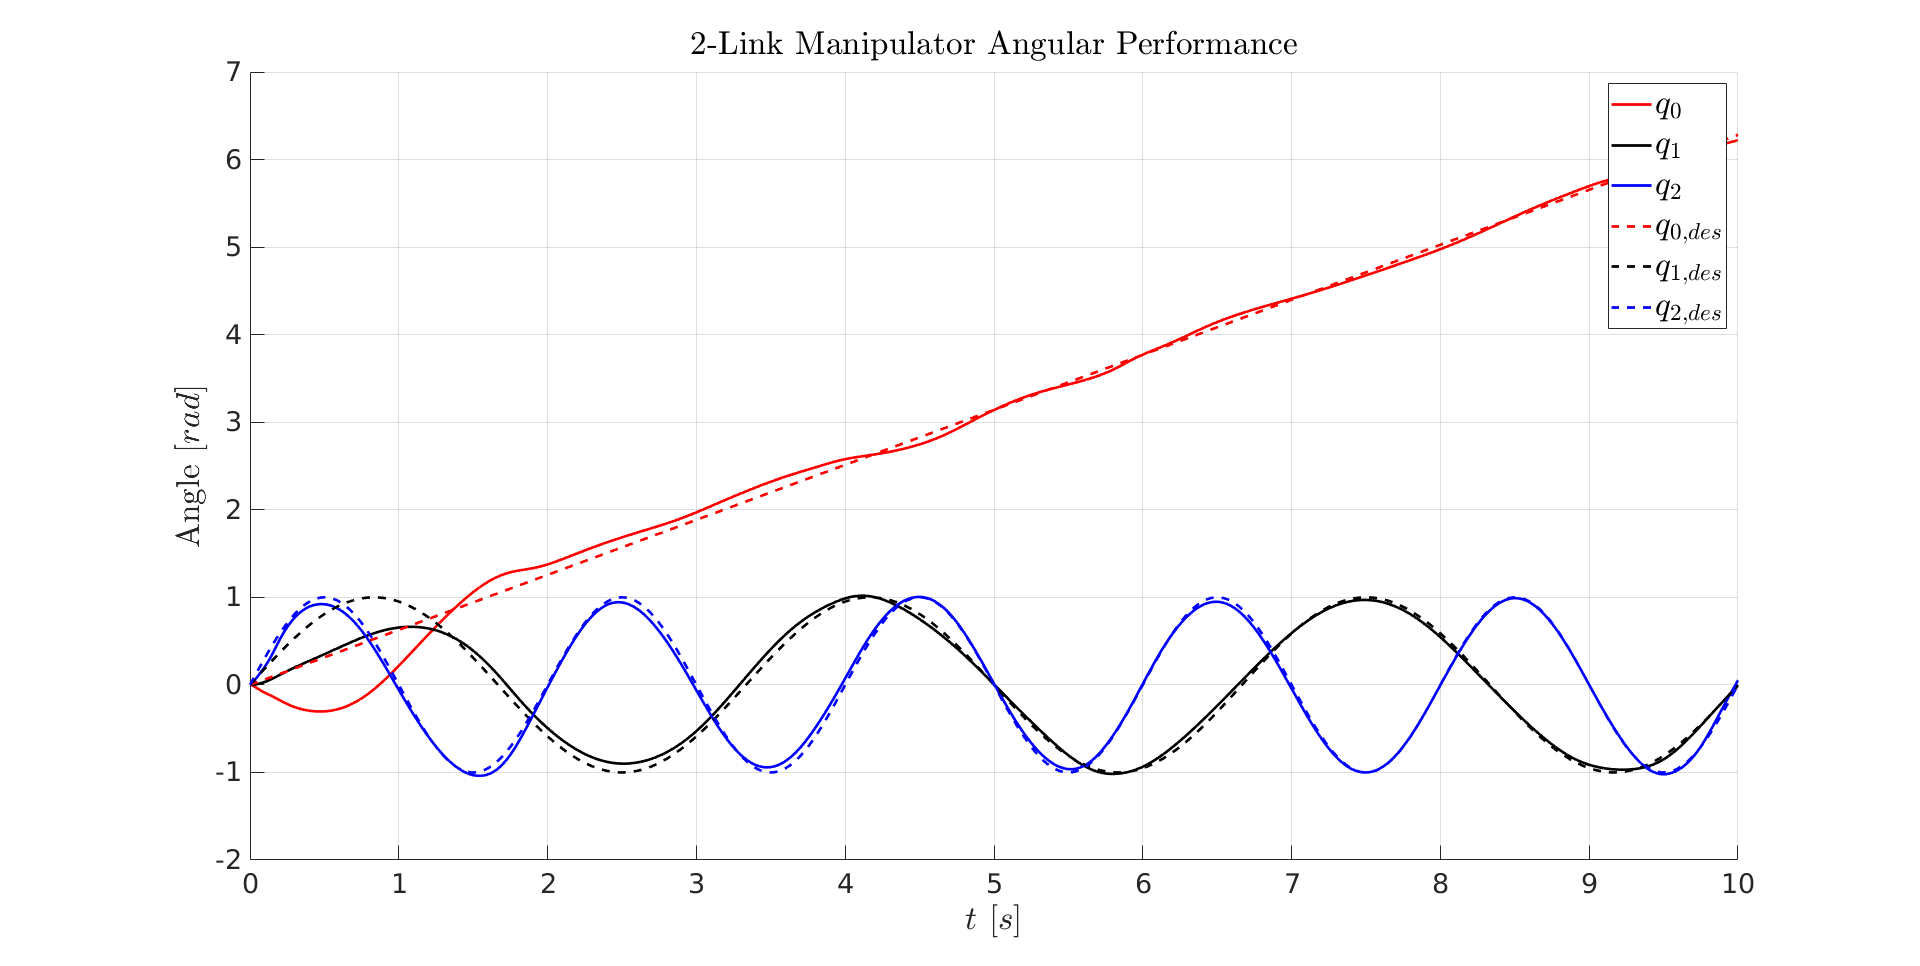
\includegraphics[width=0.9\textwidth]{ad_ang_2.png}
	\caption{This is a tiger.}
\end{figure*}

\begin{figure*}[]
	\centering
	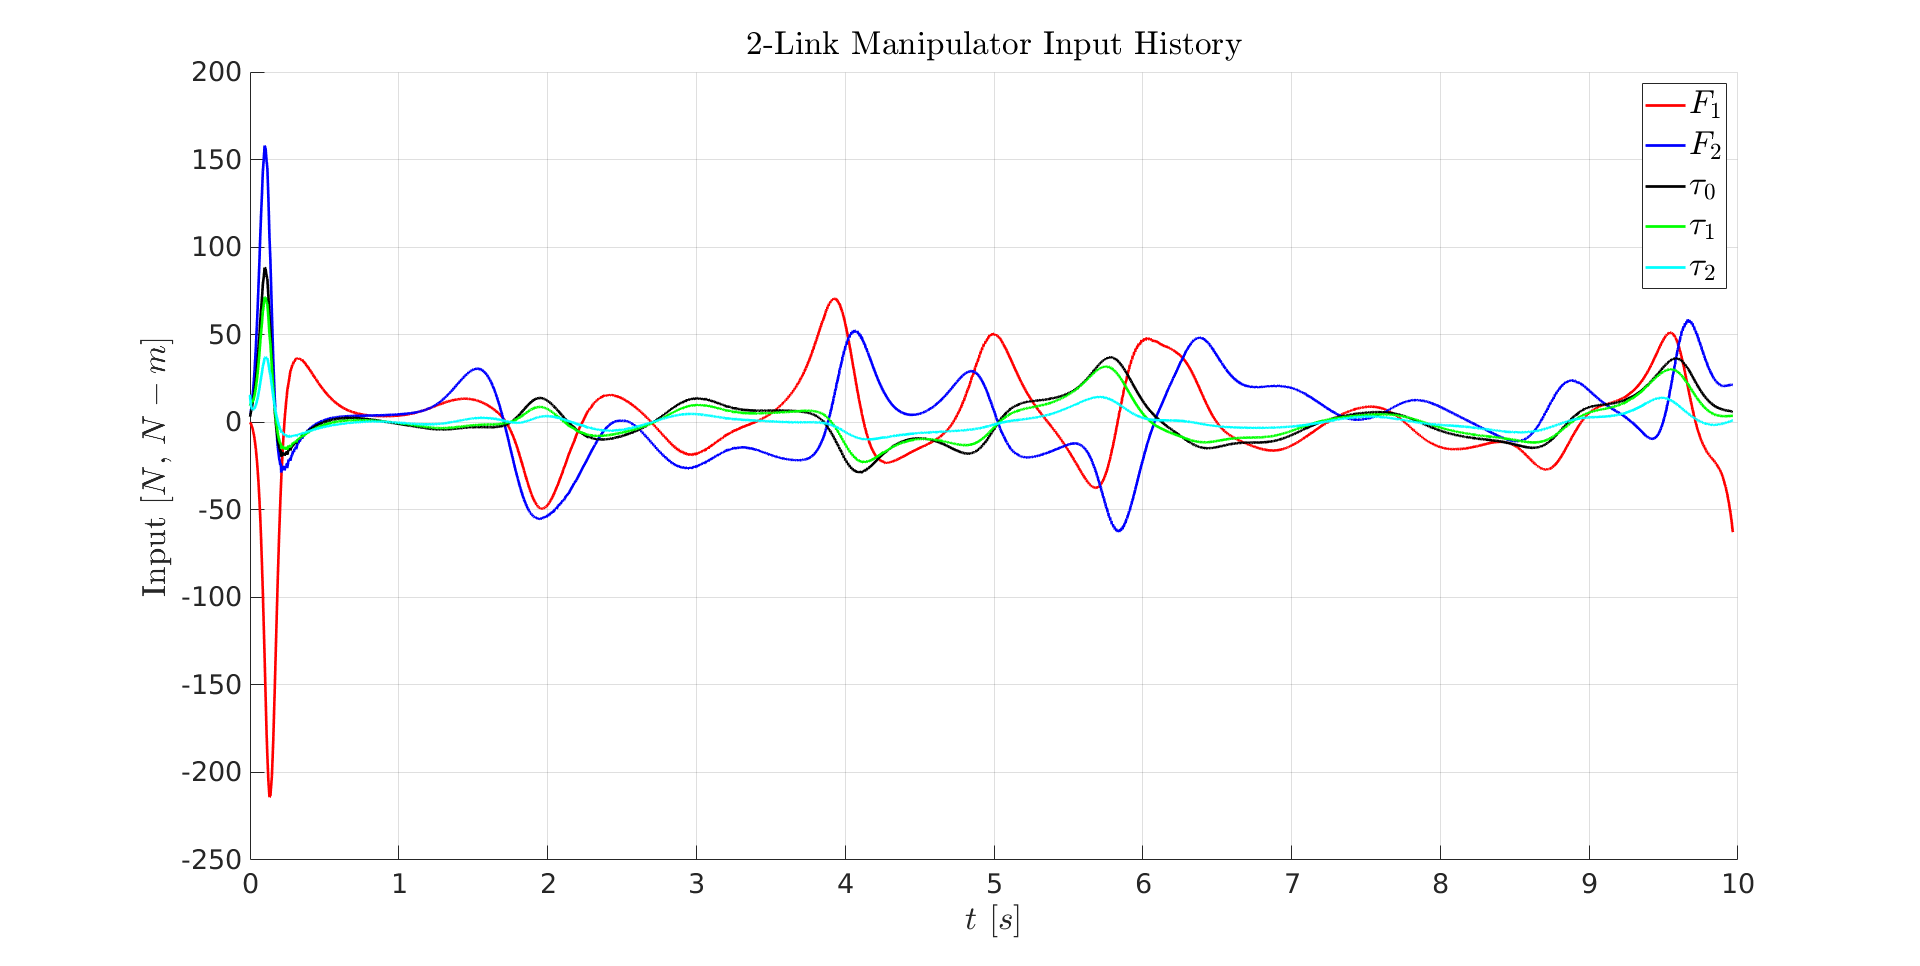
\includegraphics[width=0.9\textwidth]{ad_u_2.png}
	\caption{This is a tiger.}
\end{figure*}
\begin{figure*}[]
	\centering
	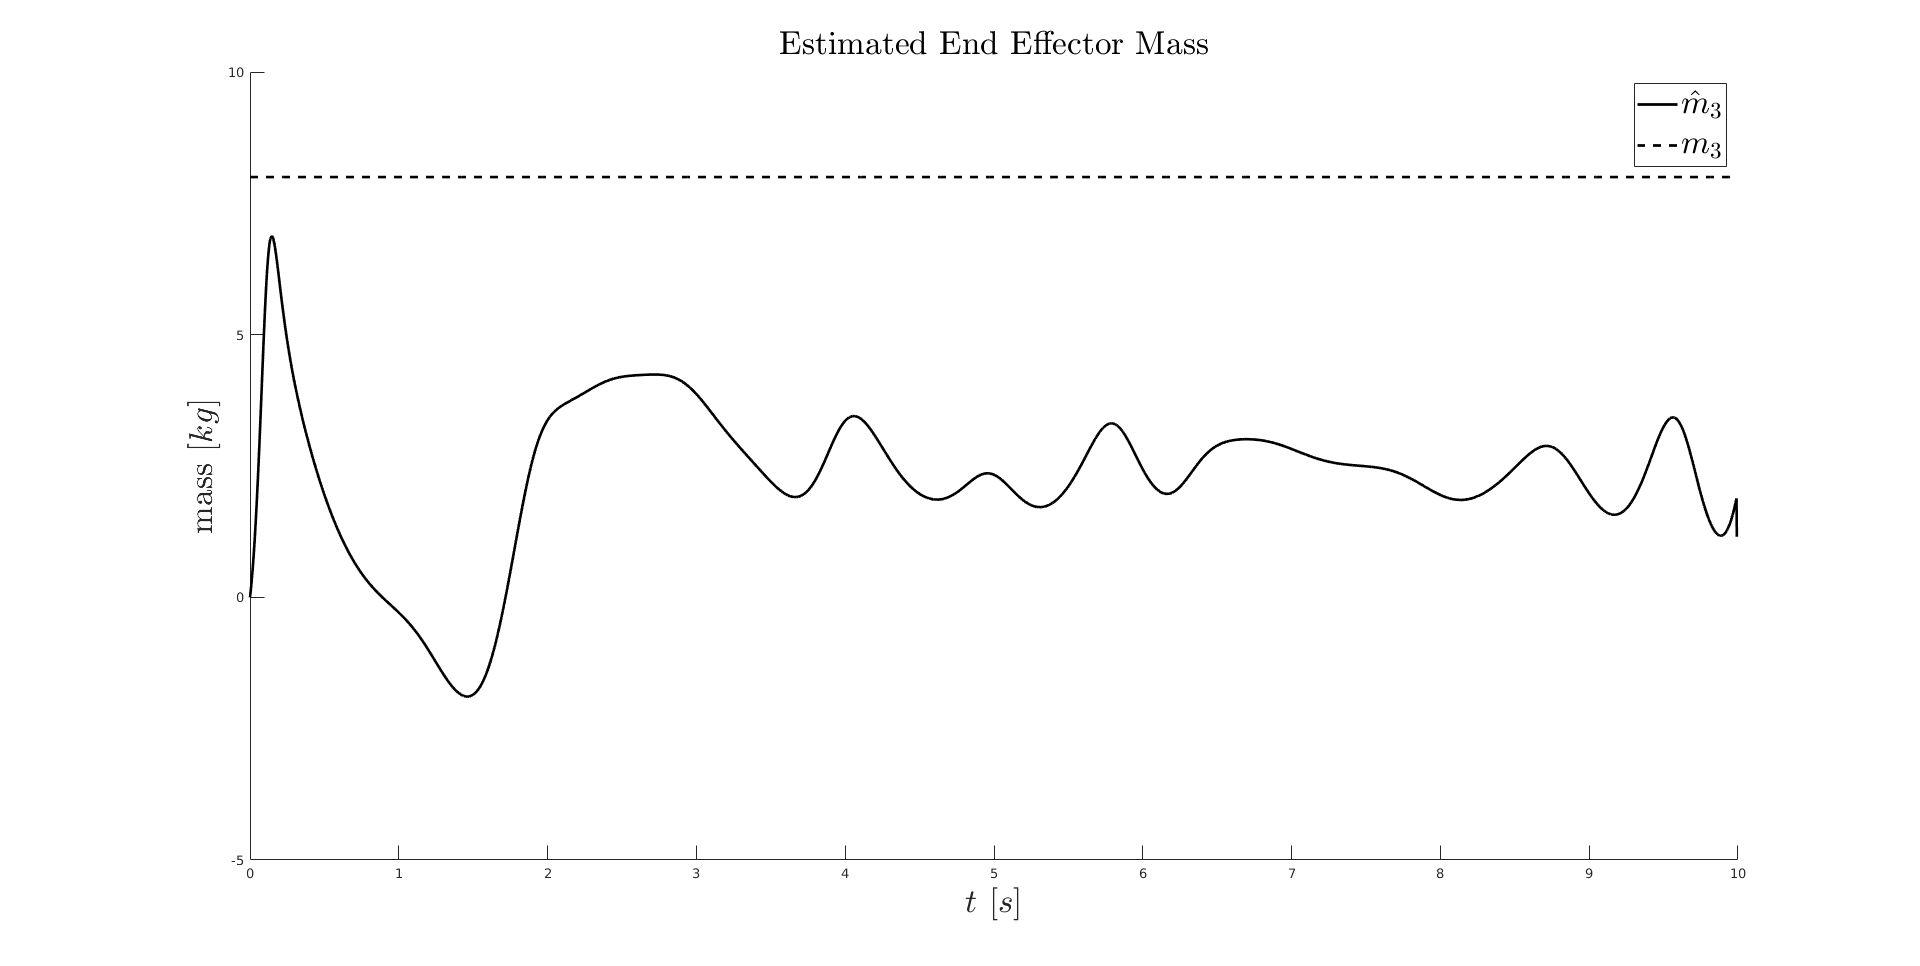
\includegraphics[width=0.9\textwidth]{ad_m_2.png}
	\caption{This is a tiger.}
\end{figure*}



\section{CONCLUSIONS}

The simulation results show

%\addtolength{\textheight}{-12cm}   % This command serves to balance the column lengths
                                  % on the last page of the document manually. It shortens
                                  % the textheight of the last page by a suitable amount.
                                  % This command does not take effect until the next page
                                  % so it should come on the page before the last. Make
                                  % sure that you do not shorten the textheight too much.

%%%%%%%%%%%%%%%%%%%%%%%%%%%%%%%%%%%%%%%%%%%%%%%%%%%%%%%%%%%%%%%%%%%%%%%%%%%%%%%%



%%%%%%%%%%%%%%%%%%%%%%%%%%%%%%%%%%%%%%%%%%%%%%%%%%%%%%%%%%%%%%%%%%%%%%%%%%%%%%%%



%%%%%%%%%%%%%%%%%%%%%%%%%%%%%%%%%%%%%%%%%%%%%%%%%%%%%%%%%%%%%%%%%%%%%%%%%%%%%%%%
\section*{APPENDIX}



\section*{ACKNOWLEDGMENT}




%%%%%%%%%%%%%%%%%%%%%%%%%%%%%%%%%%%%%%%%%%%%%%%%%%%%%%%%%%%%%%%%%%%%%%%%%%%%%%%%

\bibliography{/home/albee/documents/Shared/research/mendeley-bibtex/library.bib}
\bibliographystyle{plain}
	
\end{document}
